\chapter{Results}
\label{chap:results}

All results are obtained on a PC with an AMD FX-9590, 16 GB RAM and an AMD Radeon HD 7970. The datasets Technologiezentrum and JB\_Haus are a courtesy of rmData\cite{rmdata}. Section \ref{sec:shape_detection_results} shows benchmarks for the shape detection and verifies the capability of the user-guided shape detection to be performed in interactive time. Section \ref{sec:interaction_results} provides a set of screenshots that show the workflow of the user-guided interactions on a different data set. 


\section{Shape Detection Results}
\label{sec:shape_detection_results}

The interactions proposed in this thesis heavily rely on the ability to detect meaningful shapes for regions of interest within interactive time. Therefore it must be assured that the shape detection provides results within interactive time such that the detected shapes can be used immediately for interactions. Section \ref{sec:shape_detection_performance} discusses the performance obtained in the test computer. Section \ref{sec:shape_detection_problems} discusses flaws of the shape detection algorithm that occurred while implementing this thesis.


\subsection{Performance}

\label{sec:shape_detection_performance}

The goal of the \textit{user-guided shape detection} is to provide meaningful results within interactive time, such that detected shapes can be used to support interactions immediately. The capabilities of the implementation by Schnabel et al. \cite{schnabel-2007-software} are benchmarked on three different datasets: 

\begin{center}
\begin{tabular}{ l | r | r | r }
																	& \textbf{\#Points}	& \textbf{\#Nodes}	& \textbf{max. LoD} \\
    \hline
  JB\_Haus.pts                    & 620.722           & 440             	& 15 \\
  Technologiezentrum\_Teil1.pts   & 11.762.924        & 8863             	& 15 \\
  Synthetic\_Primitives.pts     	& 472.000           & 315               & 5 \\
    
\end{tabular}
\end{center}

The tests are performed without user interaction. Instead, all octree nodes are collected and fed into the shape detection routine sequentially to retrieve results for each node of the point cloud. Therefore, the shape detection is performed for the complete point cloud for each level-of-detail. Each octree node contains at most 5000 points. The results are averaged over five runs. Table \ref{table:schnabel_benchmarks} shows the results averaged over all nodes. It can be seen that detecting planes only is significantly faster than detecting all types of primitive shapes. However, detecting all types of primitive shapes still produces results within interactive time. The synthetic point cloud is constructed from a set of primitives that are discretized to point sets, such that all types of primitives exist. 

\begin{table}
    \centering
    \begin{tabular}{ l || r | r | r || r | r | r}
            &\multicolumn{3}{c||}{\textbf{\#Shapes}} & \multicolumn{3}{c}{\textbf{Time (s)}}\\
            &\textbf{min} & \textbf{max} & \textbf{avg}  & \textbf{min} & \textbf{max} & \textbf{avg}  \\
            \hline
            JB\_Haus*           & 0 & 6  & 1.31 & 0.000026 & 0.578664 & 0.022396 \\
            JB\_Haus            & 0 & 6  & 1.40 & 0.000024 & 0.741384 & 0.093264 \\
            Technologiezentrum*	& 0 & 10 & 1.18 & 0.000023 & 0.440614 & 0.018781 \\
            Technologiezentrum  & 0 & 10 & 1.19 & 0.000024 & 0.991554 & 0.083180 \\
            Synthetic*          & 0 & 7  & 1.89 & 0.000026 & 0.440064 & 0.029779 \\
            Synthetic           & 0 & 7  & 1.24 & 0.000024 & 0.753345 & 0.136474 \\
        \end{tabular}
    \caption[Shape-detection performance measure for different datasets]
		{Performance measures for the different datasets averaged over all nodes. The number of shapes and duration are listed as minimum, maximum and average. Each dataset is benchmarked using plane detection only (items with *), as well as detecting all types of primitive shapes. }
    \label{table:schnabel_benchmarks}
\end{table}


\begin{figure}[h]
    \centering
    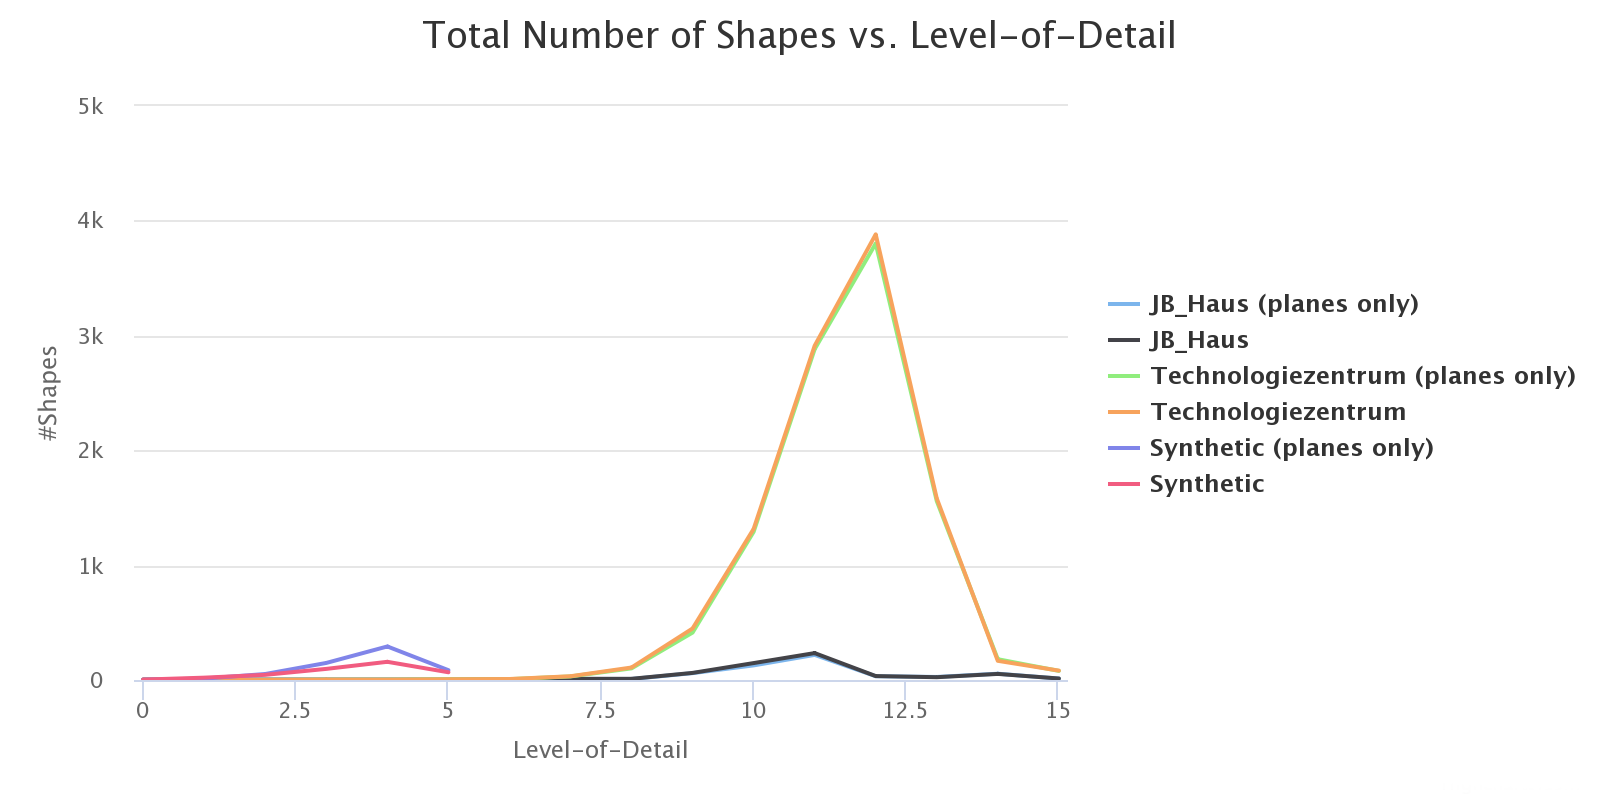
\includegraphics[width=1\textwidth]{Results/shapes_total_vs_lod.png}
    \caption[Plot of the total number of shapes vs. to the level-of-detail of the node]
		{This figure shows a plot of the total number of shapes vs. the level-of-detail of the node. All values are averaged over all nodes that share the same level-of-detail.}
    \label{fig:shapes_total_vs_lod}
\end{figure}

\begin{figure}[h]
    \centering
    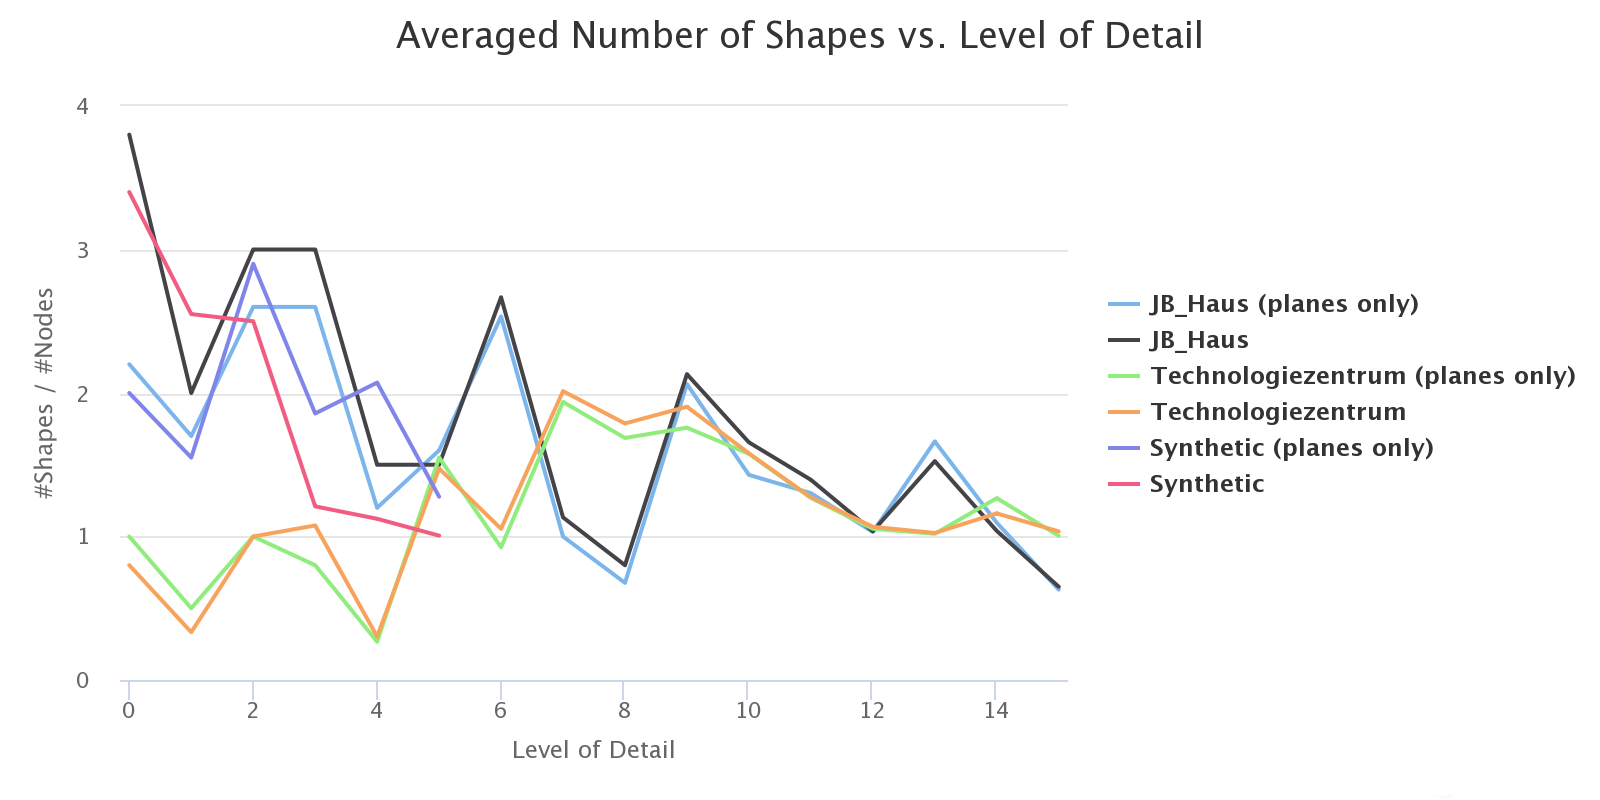
\includegraphics[width=1\textwidth]{Results/shapes_averaged_vs_lod.png}
    \caption[Plot of the average number of shapes per node vs. the level-of-detail of the node]
		{Plot of the average number of shapes per node vs. the level-of-detail of the node. All values are averaged over all nodes that share the same level-of-detail.}
    \label{fig:shapes_averaged_vs_lod}
\end{figure}

\begin{figure}[h]
    \centering
    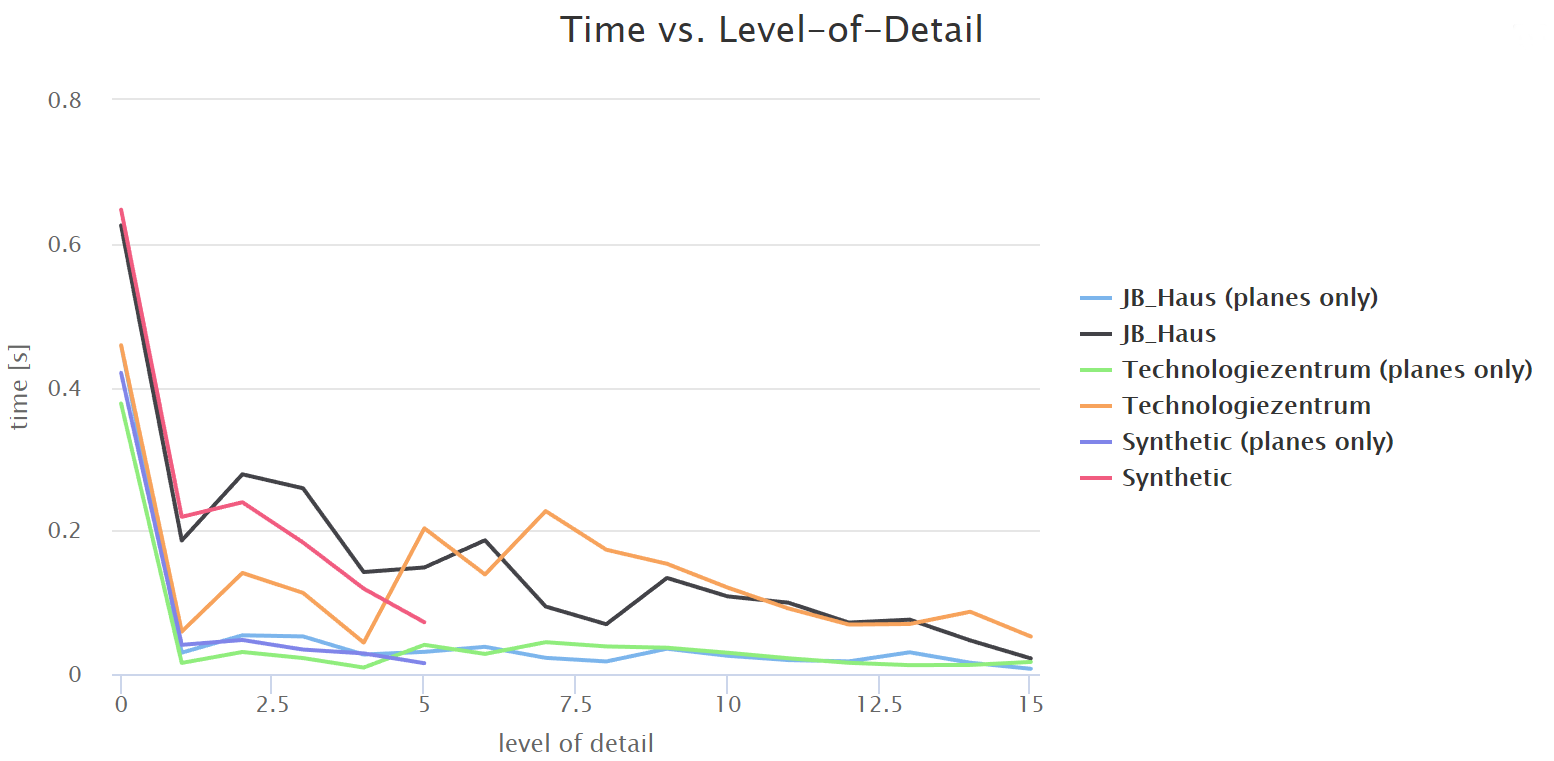
\includegraphics[width=1\textwidth]{Results/time_vs_lod.png}
    \caption[Plot of the number of shapes vs. the computation time]
		{This figure shows a plot of the number of shapes vs. the computation time. All values are averaged over all nodes that share the same level-of-detail.}
    \label{fig:time_vs_lod}
\end{figure}


Figure \ref{fig:shapes_total_vs_lod} shows the total number of shapes per level-of-detail. All three datasets share an increase in the number of shapes in the third quarter before a rapid decline for the highest level-of-detail. Figure \ref{fig:shapes_averaged_vs_lod} shows the number of shapes divided by the number of nodes per level-of-detail. Both figures emphasize that the majority of shapes is not found in the highest level-of-detail. Reasons for this is that many nodes only contain a handful of points or only contain a single structure. 
\\

Figure \ref{fig:time_vs_lod} shows the calculation time compared to the level-of-detail. Shape detection for smaller, more dense nodes take less time than for larger nodes with lower level-of-detail as in larger nodes, usually more shapes are found. 


\subsection{Problems and undesired Behavior}
\label{sec:shape_detection_problems}
A problem with the shape detection implementation by Schnabel et al. \cite{schnabel-2007-software} are reoccurring non-terminations for some octree nodes, causing the shape detection coroutine to stall. To circumvent this problem, all shape detection tasks that are dispatched to the \verb|sequential computation applicator| are assigned a timeout value of one second, after which the computation is interrupted. 
\\
Another reoccurring problem with the shape detection is the plausibility of detected shapes. The RANSAC options guarantee that shapes are found that fit the local geometry within a certain margin, $\alpha$ for the normal's angle and $\epsilon$ for the distance the shape. So within theses two parameters, the shape is considered to be valid. However, certain constellations of points allow the shape detection to produce non-plausible results that are accurate regarding the RANSAC parameters but are not plausible to the eye. A prominent example is a torus that is fitted onto a section that describes a cylinder. The major radius of the torus is of such dimensions that the local cylinder fits within the curvature of the torus. Thus, a torus is detected, rather than the simpler cylinder. Figure \ref{fig:missfittedTorus} shows this behavior within an example scene that consists multiple primitives. Figure \ref{fig:missfittedTorus2} shows the size of the detected torus. 
\\
Such non-plausible shapes can exist due to the density-controlled $\epsilon$ parameter that weakens the margin for octree nodes of larger volume. Even within a node, the density can strongly vary for different regions. 

\begin{figure}[h]
\centering
\subcaptionbox{ \label{fig:missfittedTorus1}}{%
  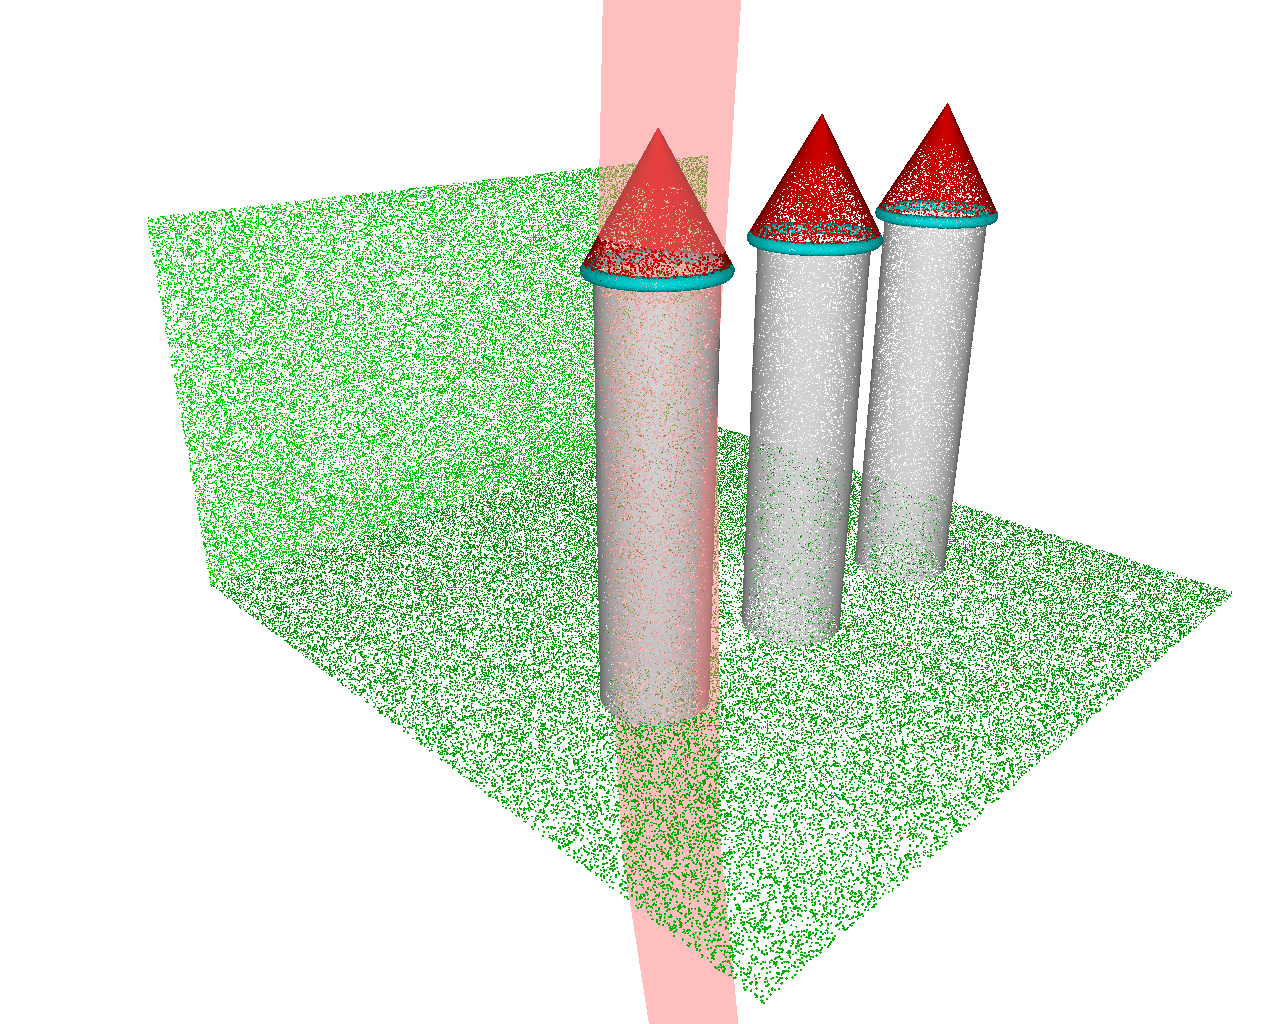
\includegraphics[width=0.49\textwidth]{Results/missfittedTorus1.png}%7
  }%\par\medskip
\subcaptionbox{ \label{fig:missfittedTorus2}}{%
  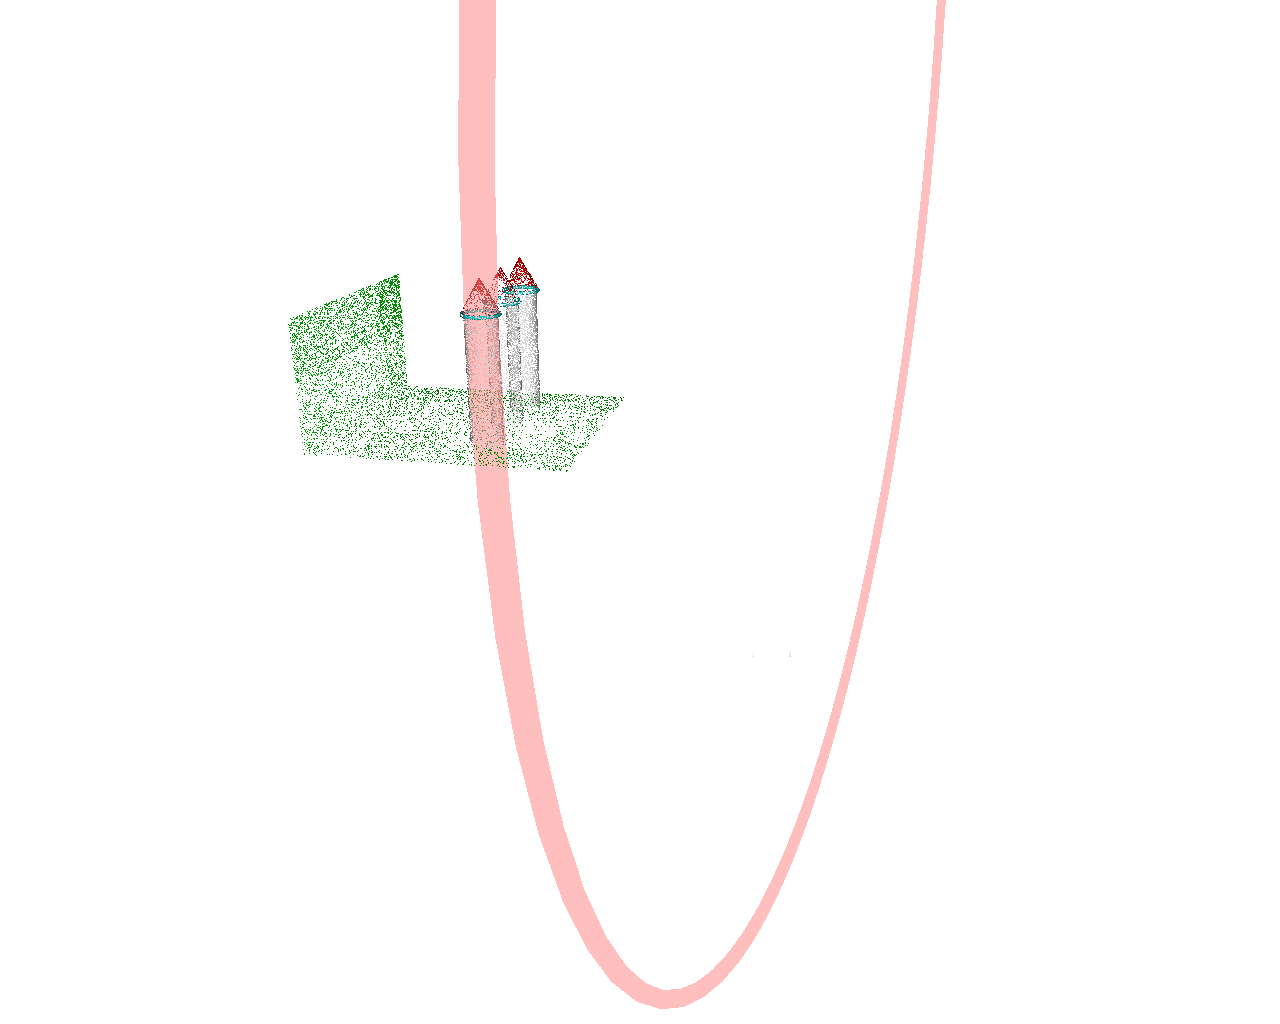
\includegraphics[width=0.49\textwidth]{Results/missfittedTorus2.png}%
  }      
\caption[Implausible torus is detected instead of a more plausible cylinder. ]
{This figure shows a cylinder from the synthetic point cloud whose points are classified as a torus instead of a cylinder. Even tough the points fit the torus, determined by the RANSAC options, the result is not plausible, since the user would expect a cylinder for this constellation of points. }
\label{fig:missfittedTorus}
\end{figure}


\section{Interaction Performance}

	\begin{center}
	\begin{tabular}{ r| r | r }
			\textbf{min}	& \textbf{max}	& \textbf{avg} \\
			\hline
			0.348200 & 39.929400 & 3.281752\\
	13.402100 & 148.346100 & 37.964309 \\
	\end{tabular}
	\caption{Benchmark Point Picking}
	\end{center}


without support: 193.628900 ; 2494.494800 ; 748.725405
with support: 191.082600 ; 923.332500 ; 437.933686

Lasso Performance lasso selection + shape-assisted lasso selection with same lasso ratio between computation time averaged ratio 1.810198

Ration between computation time: 1.810198


\subsection{Results}

This section presents results for the RANSAC shape detection performed on three data sets. The results in Figure \ref{fig:synthetic_point_cloud_results}, \ref{fig:JB_haus_results}, and \ref{fig:technologiezentrum_results} are obtained by segmenting the point clouds as a whole. Results for the interactive shape detection can be seen in Figure \ref{fig:technologiezentrum_interactive_shape_detection}. 

The synthetic test scene consists of two planes, three cylinders, three tori, and three cones.  Figure \ref{fig:synthetic_point_cloud_results} shows the synthetic point cloud, as well as the shapes that are detected within the point cloud. As the RANSAC approach randomly selects a subset of points, the results can be different for different runs. 

\begin{figure}[h]
\centering
\subcaptionbox{ \label{fig:synthetic_point_cloud}}{%
  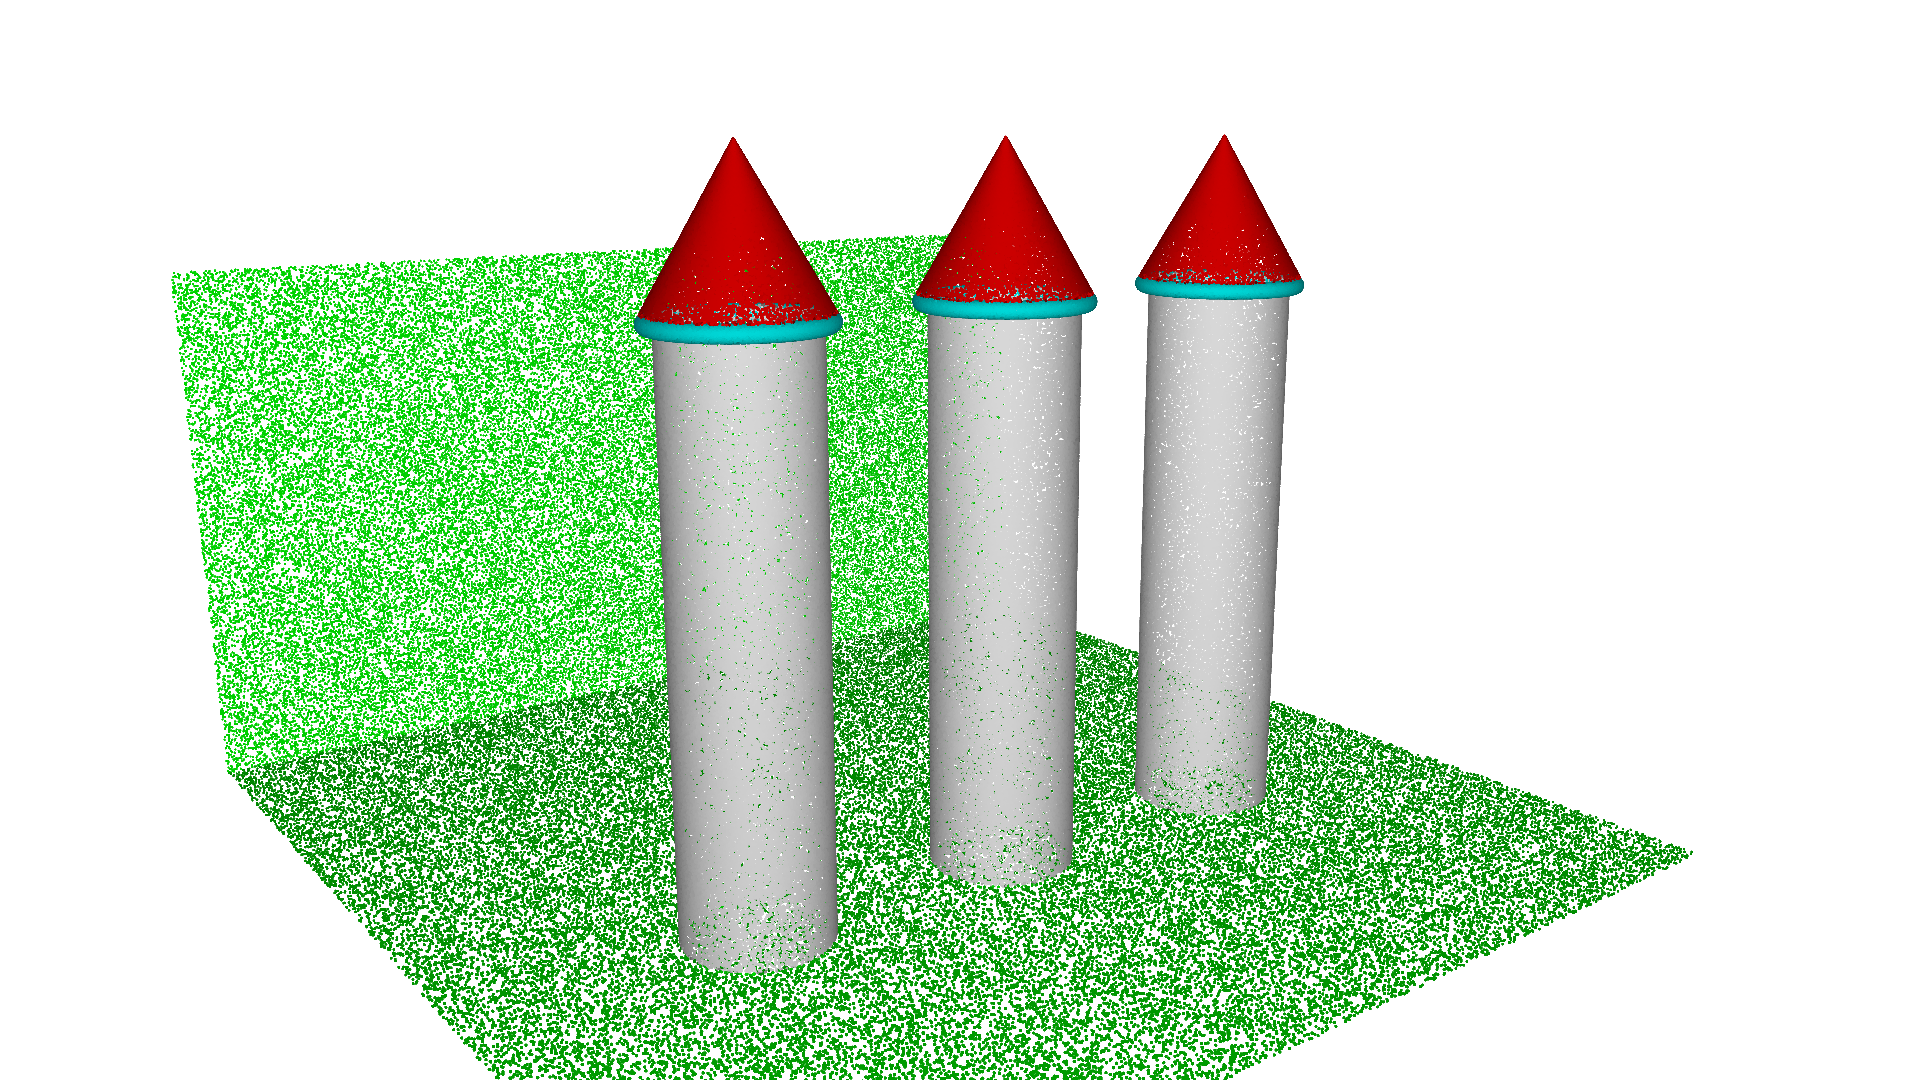
\includegraphics[width=0.7\textwidth]{Results/synthetic_point_cloud.png}%7
  }
\subcaptionbox{ \label{fig:synthetic_point_cloud_shapes}}{%
  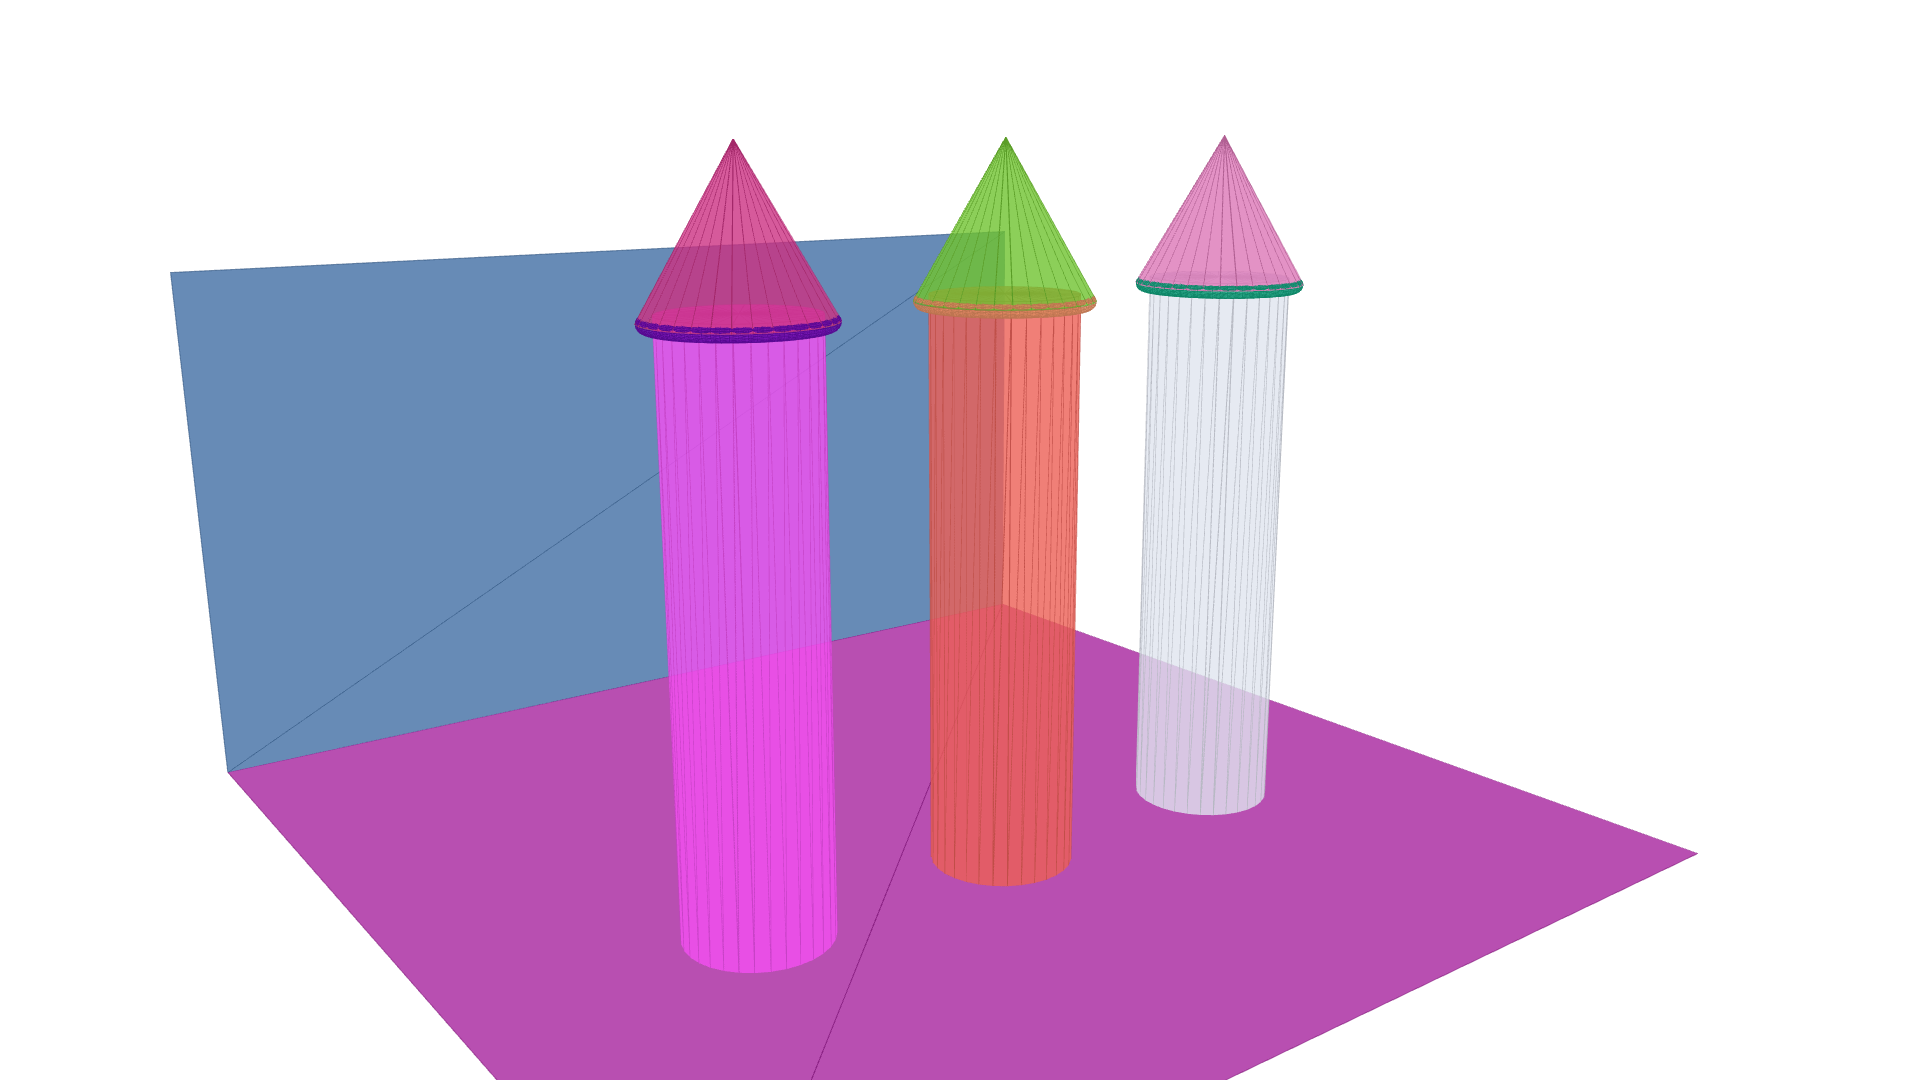
\includegraphics[width=0.7\textwidth]{Results/synthetic_point_cloud_shapes.png}%
  }
\caption[Rendering of the synthetic point cloud in (a), rendering of the detected shapes in (b)]
{(a) shows the synthetic point cloud, consisting of two planes, three cylinders, three tori, and three cones. (b) shows the detected shapes rendered as triangle meshes. For each shape in the point cloud, the RANSAC shape detection has found a suitable primitive shape. }
\label{fig:synthetic_point_cloud_results}
\end{figure}

\begin{figure}
\centering
\subcaptionbox{ \label{fig:jb_haus}}{%
  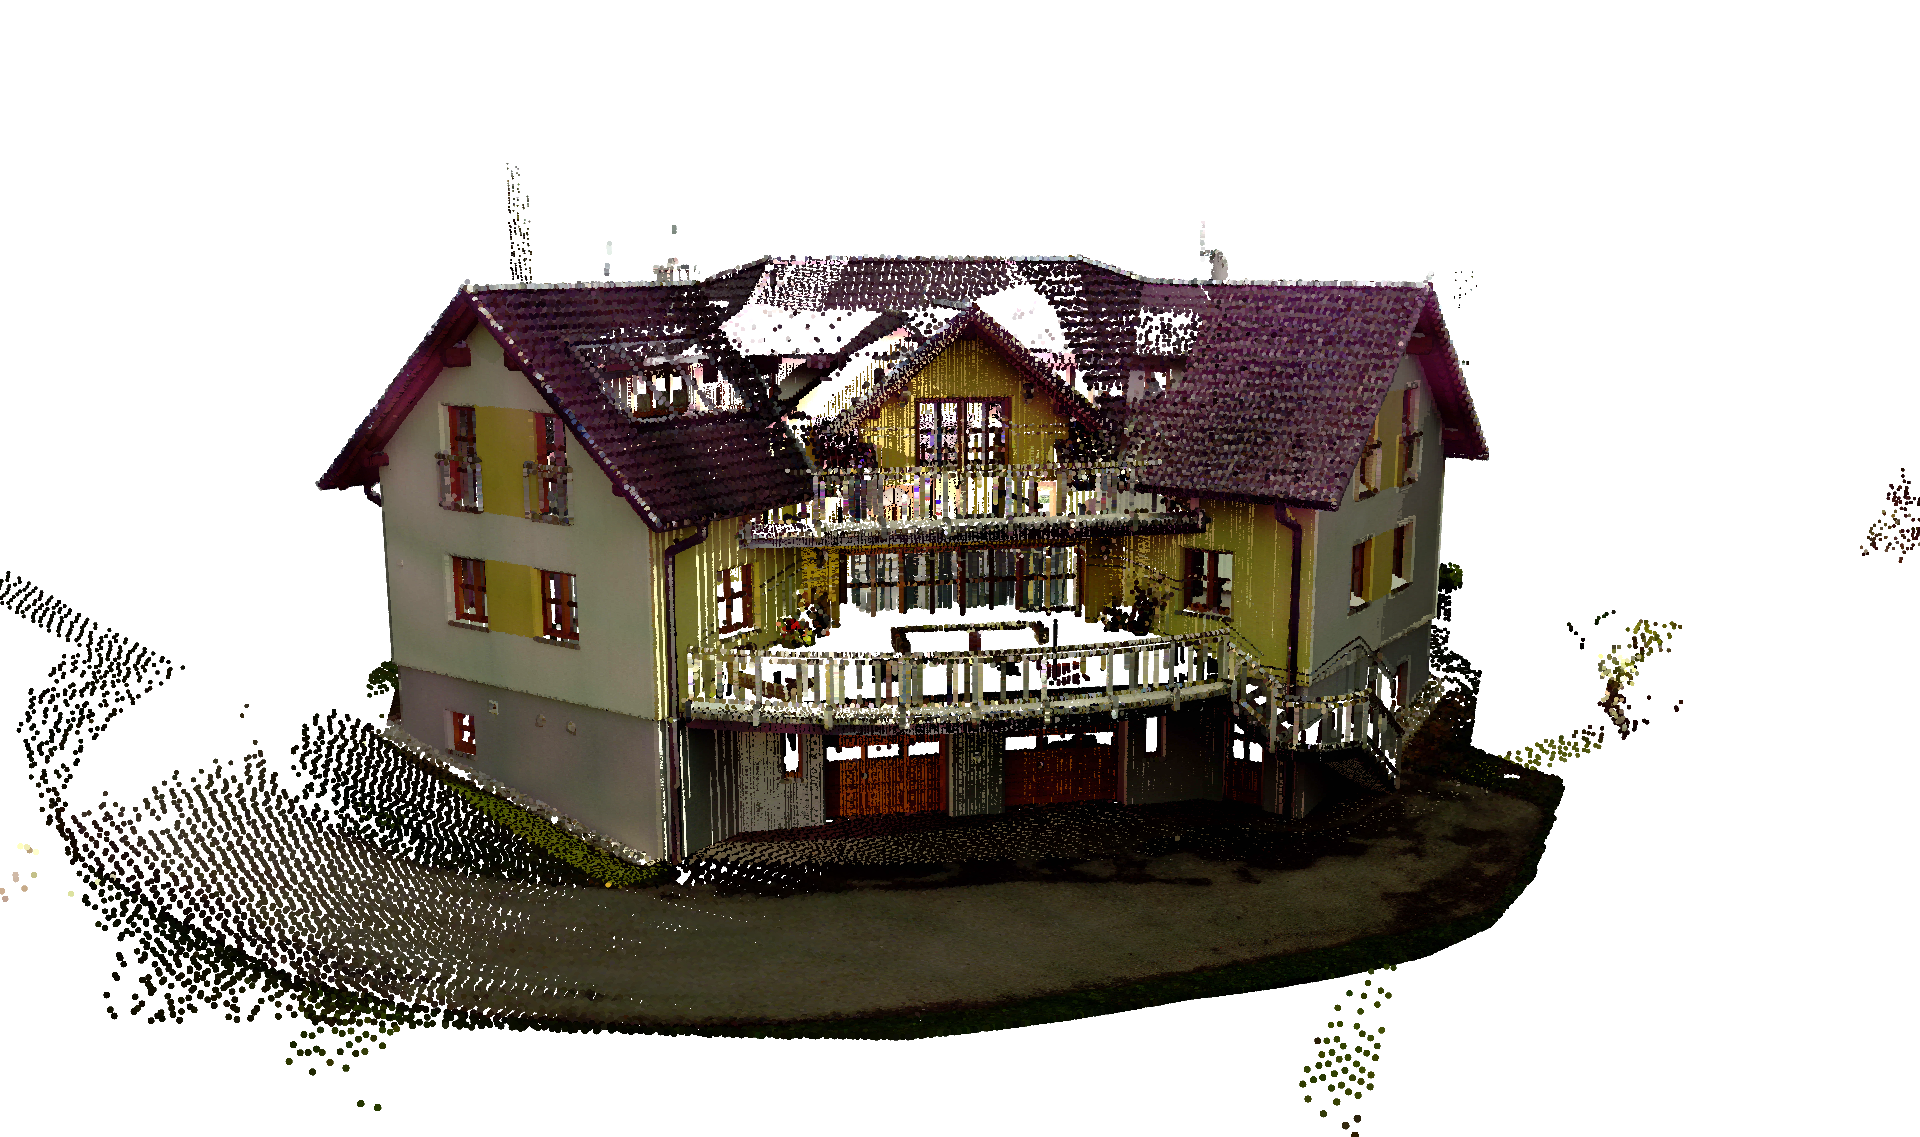
\includegraphics[width=0.7\textwidth]{Results/jb_haus.png}%7
  }
\subcaptionbox{ \label{fig:jb_haus_shapes}}{%
  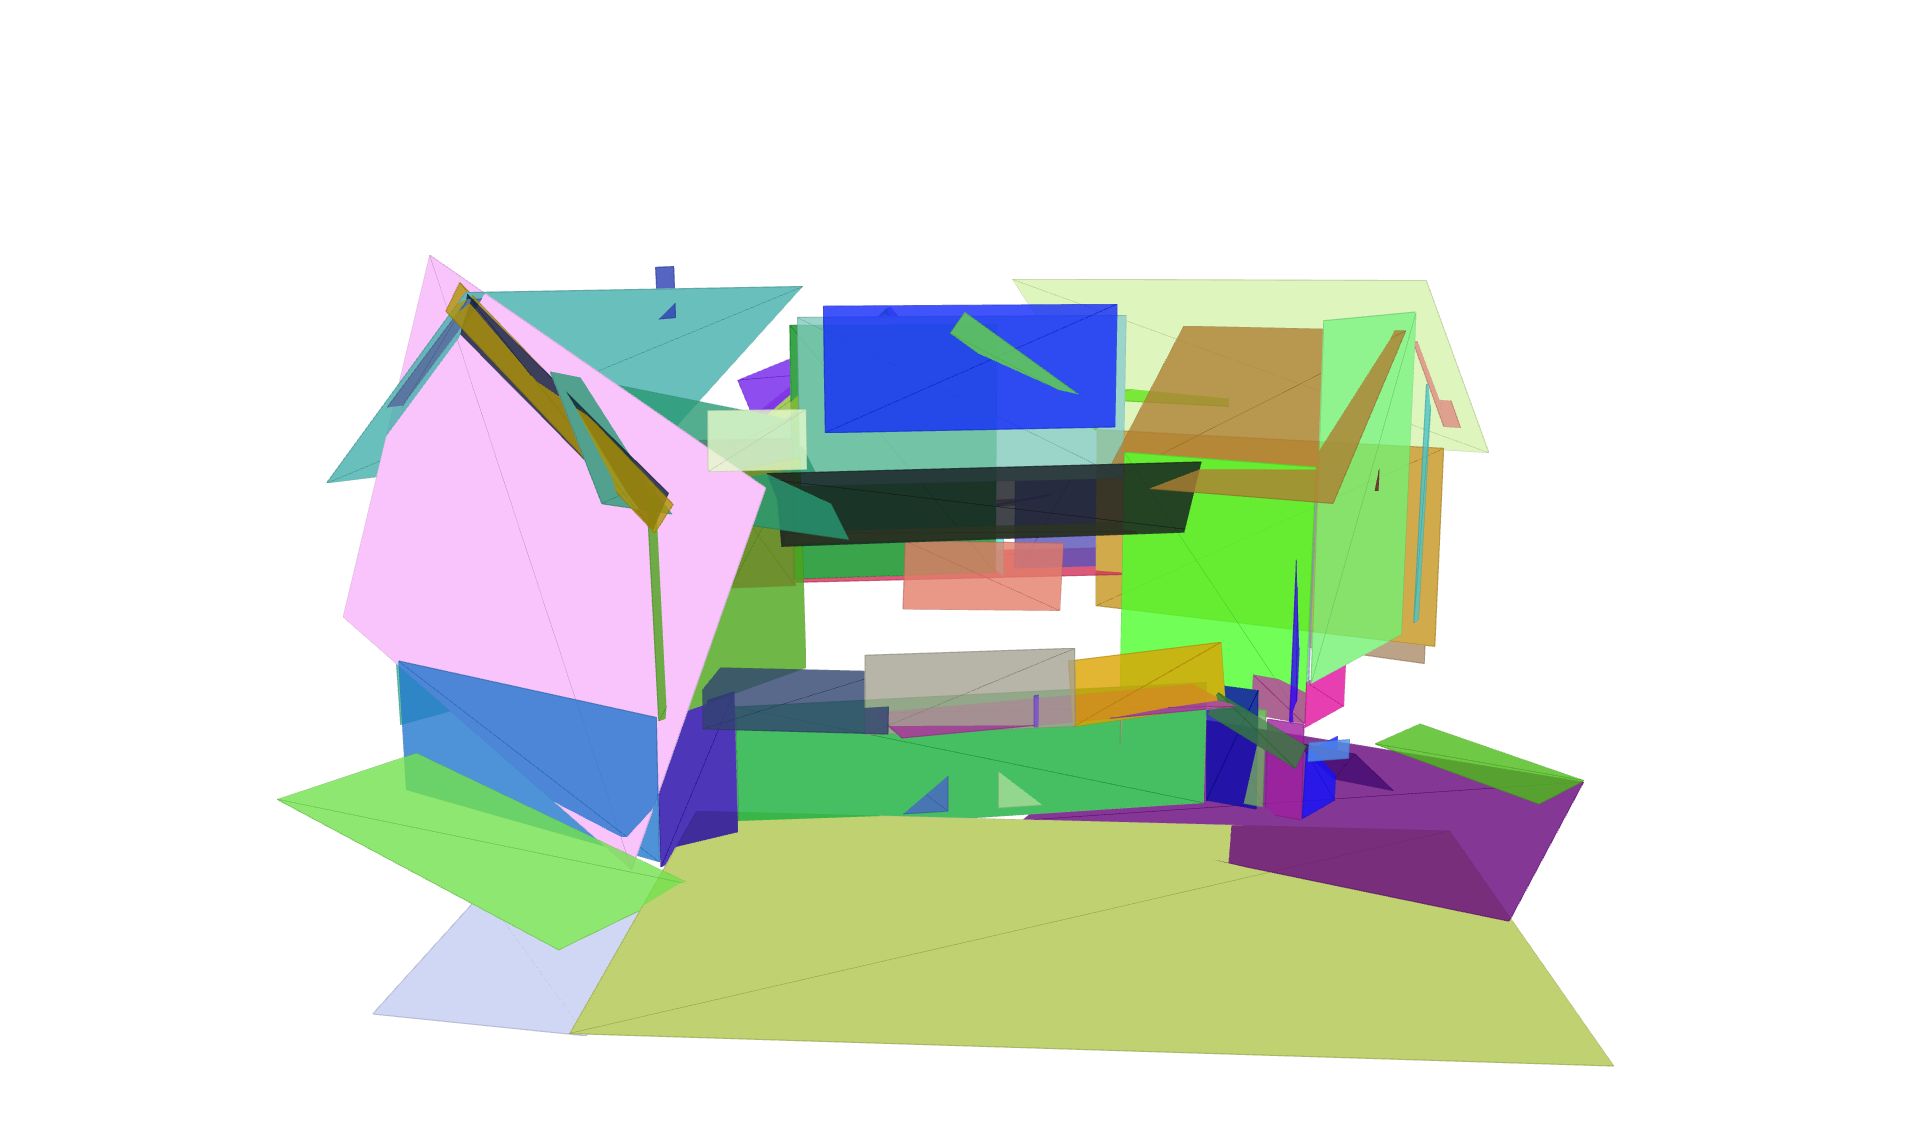
\includegraphics[width=0.7\textwidth]{Results/jb_haus_shapes.png}%
  }
\subcaptionbox{ \label{fig:jb_haus_shapes}}{%
  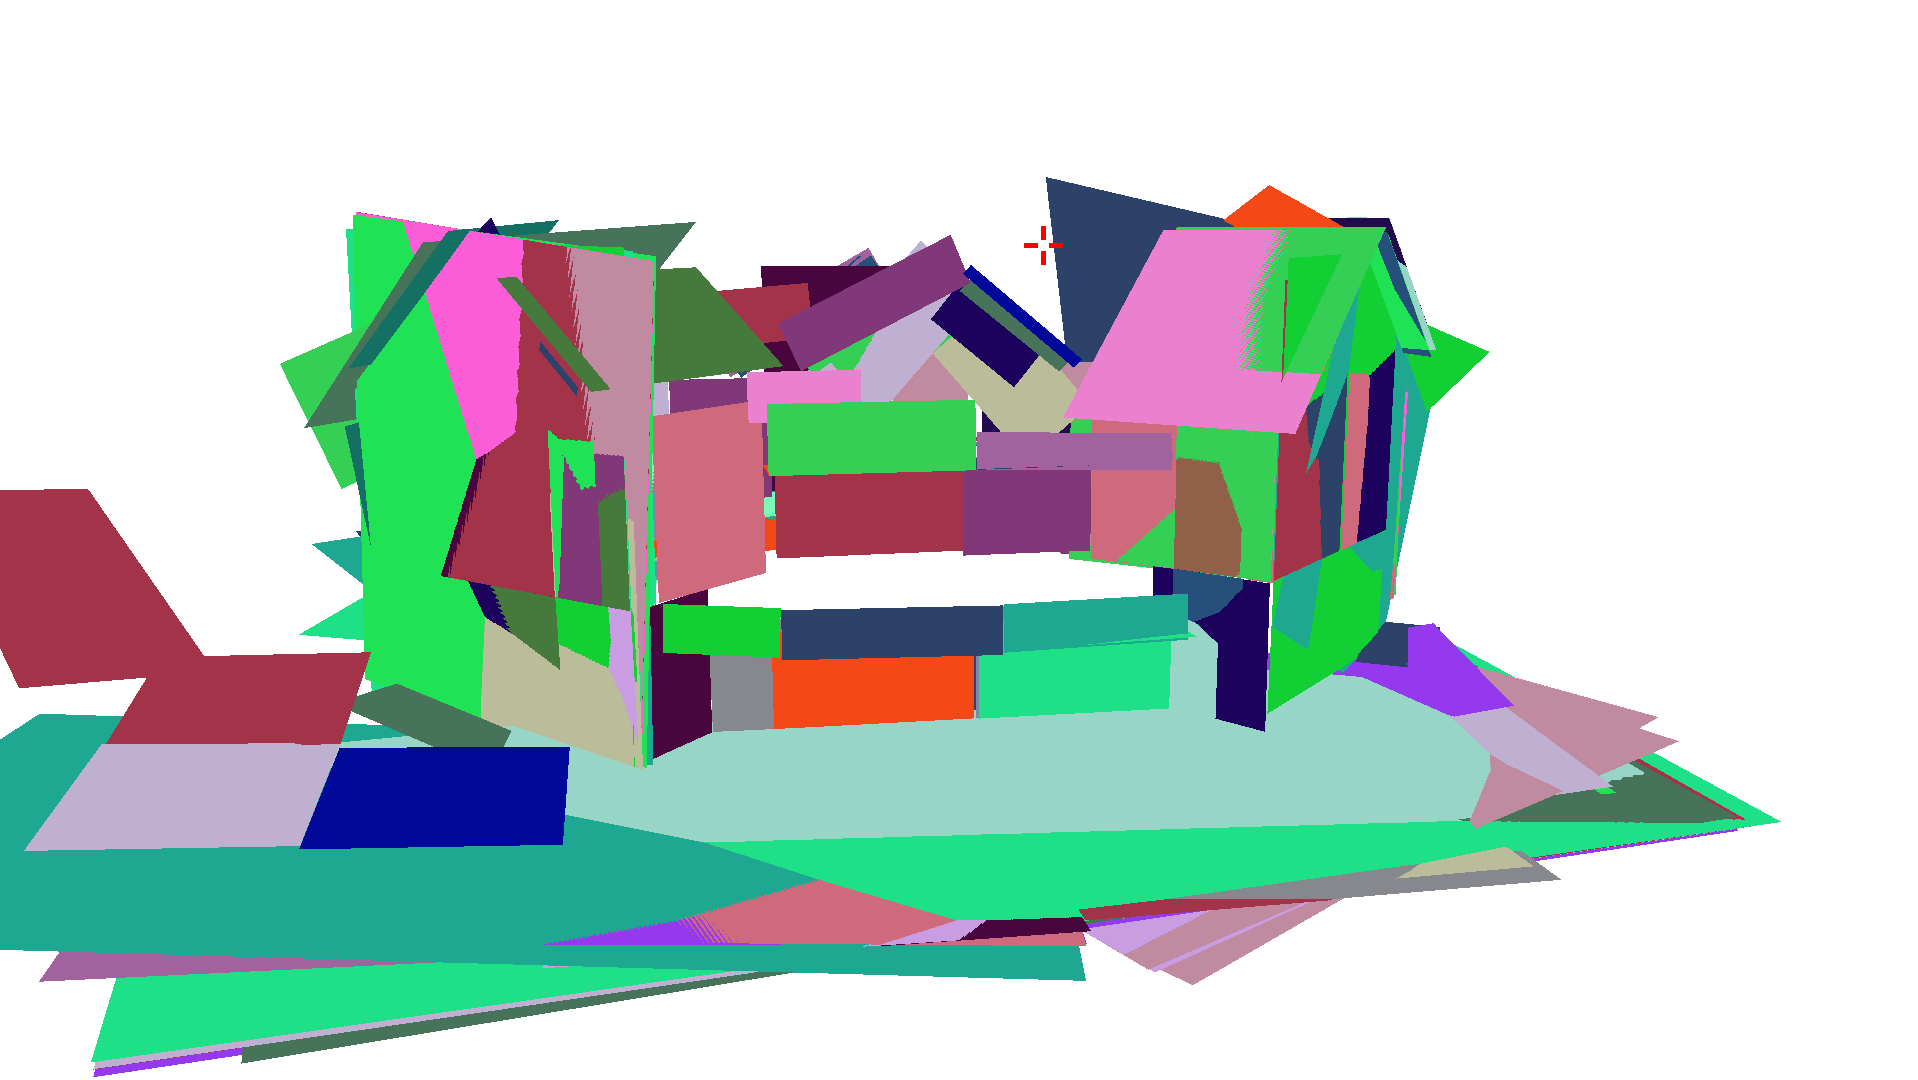
\includegraphics[width=0.7\textwidth]{Results/jb_haus_shapes_interactive.png}%
  }
\caption[Figure (a) shows a rendering og the JB\_haus dataset, (b) shows the resulting shapes of the RANSAC shape detection, (c) shows the result of the interactive shape detection. ]
{Figure (a) shows a rendering of the JB\_haus dataset, (b) shows the resulting shapes of the RANSAC shape detection, (c) shows the detected shapes using the interactive shape detection method.  }
\label{fig:JB_haus_results}
\end{figure}

\begin{figure}
\centering
\subcaptionbox{ \label{fig:technologiezentrum}}{%
  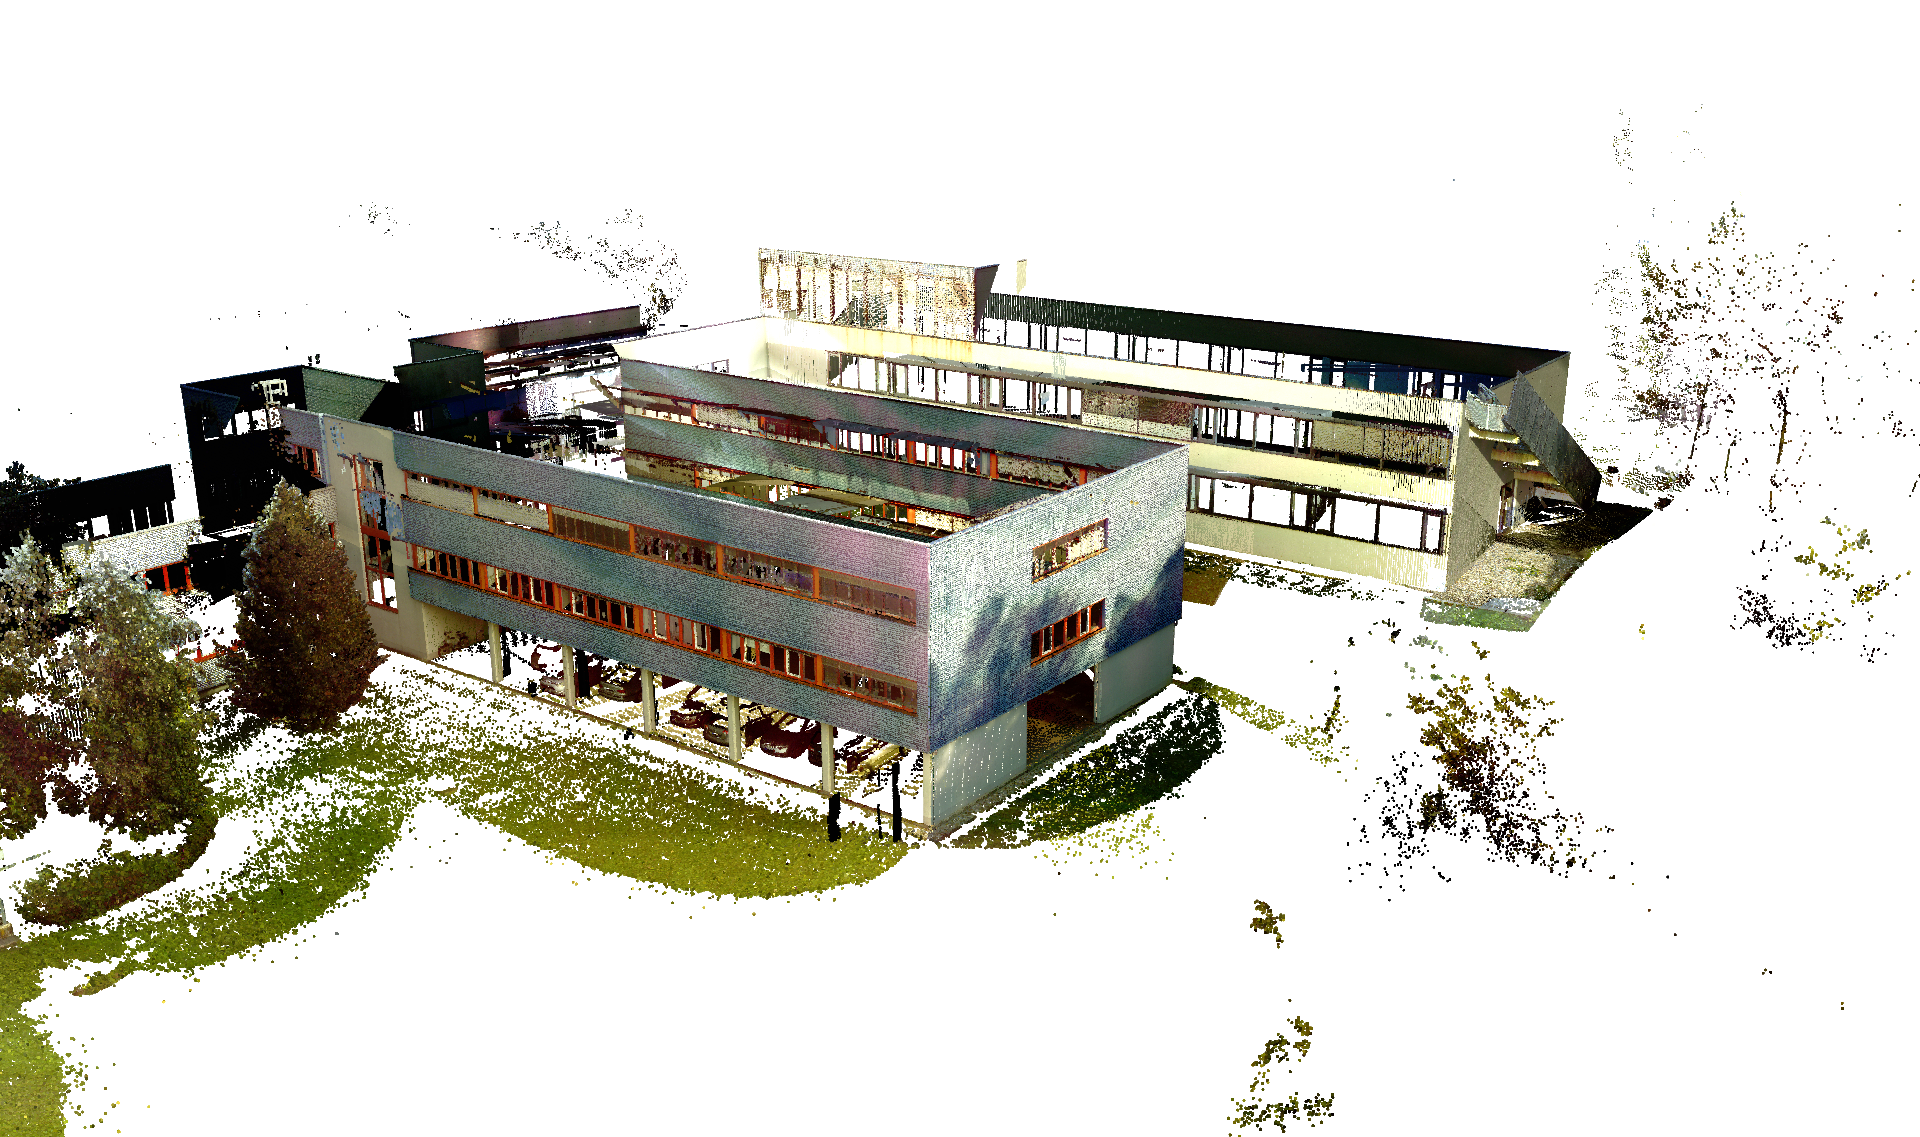
\includegraphics[width=0.7\textwidth]{Results/technologiezentrum.png}%7
  }
\subcaptionbox{ \label{fig:technologiezentrum_shapes}}{%
  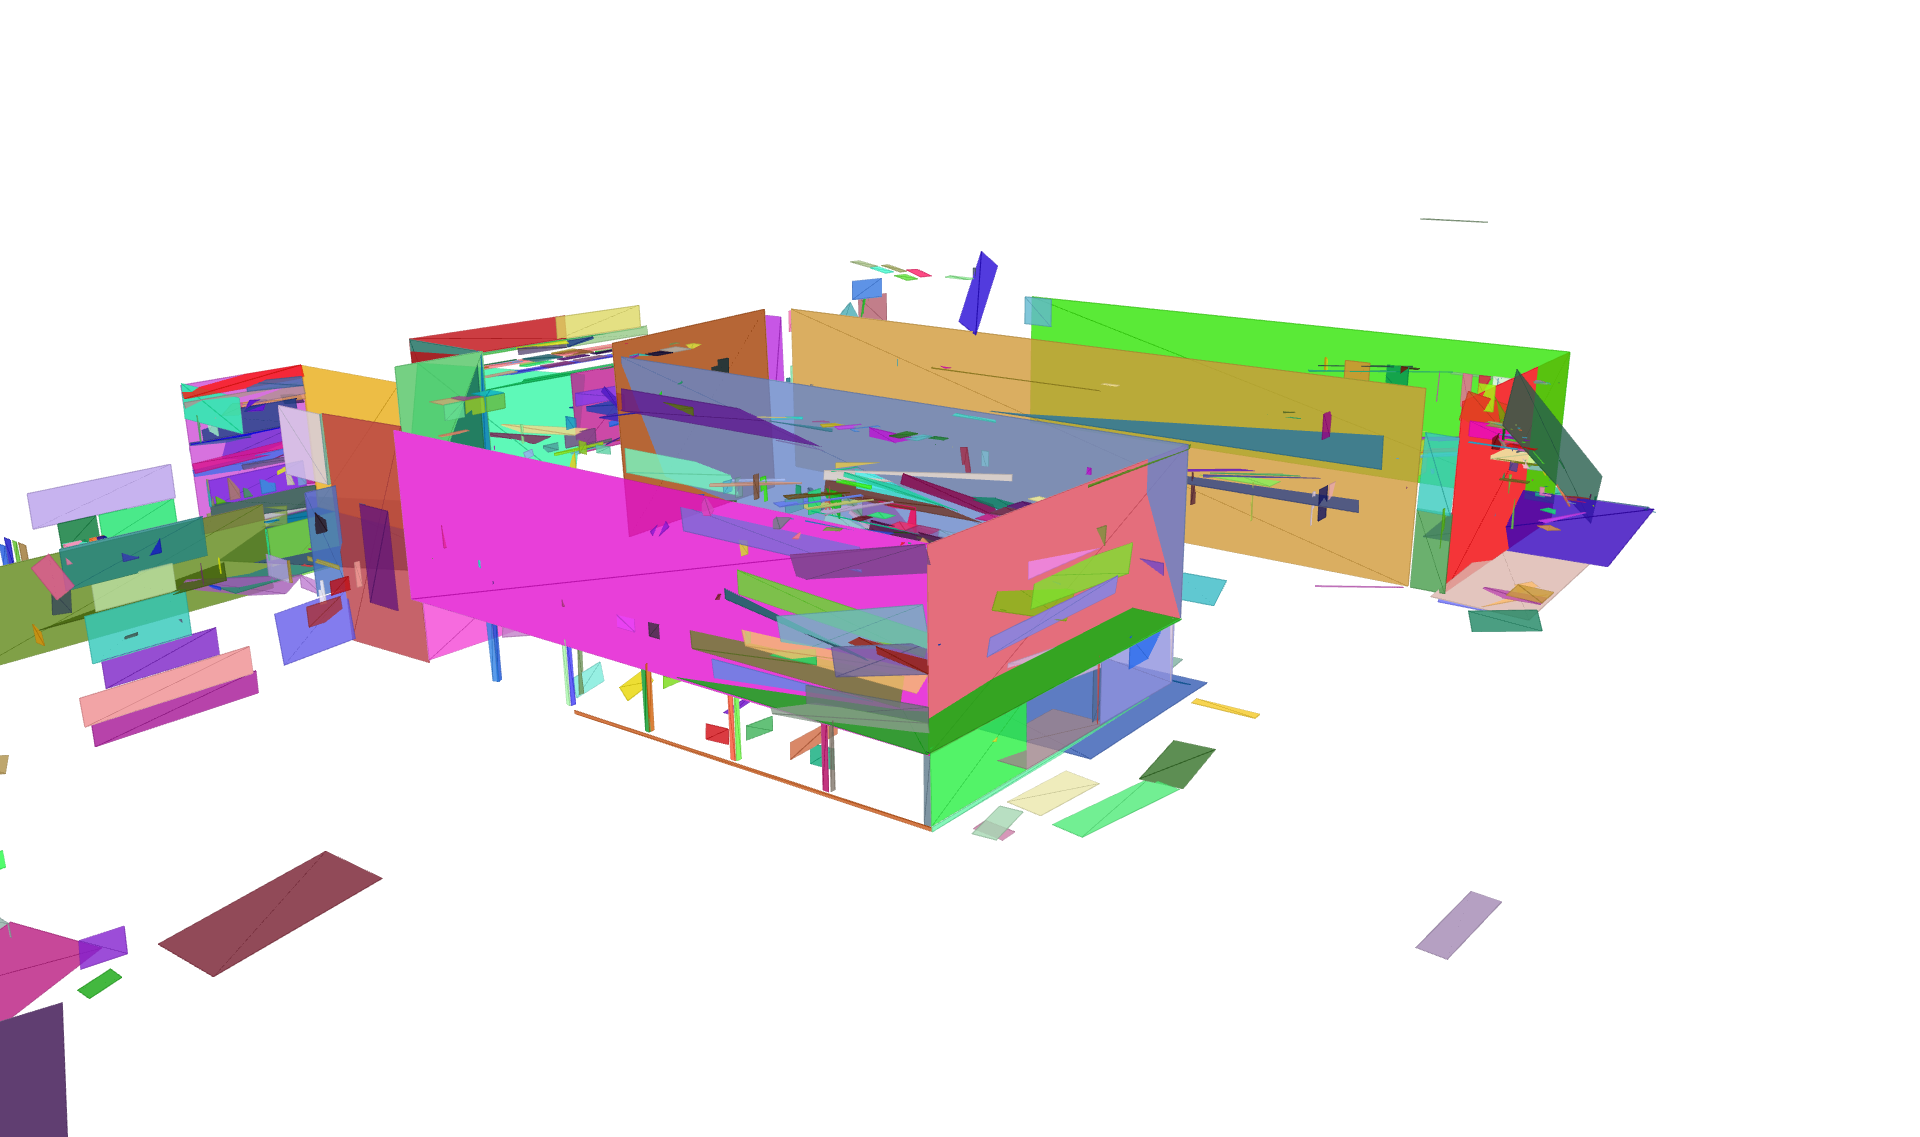
\includegraphics[width=0.7\textwidth]{Results/technologiezentrum_shapes.png}%
  }
\subcaptionbox{ \label{fig:technologiezentrum_shapes_interactive}}{%
  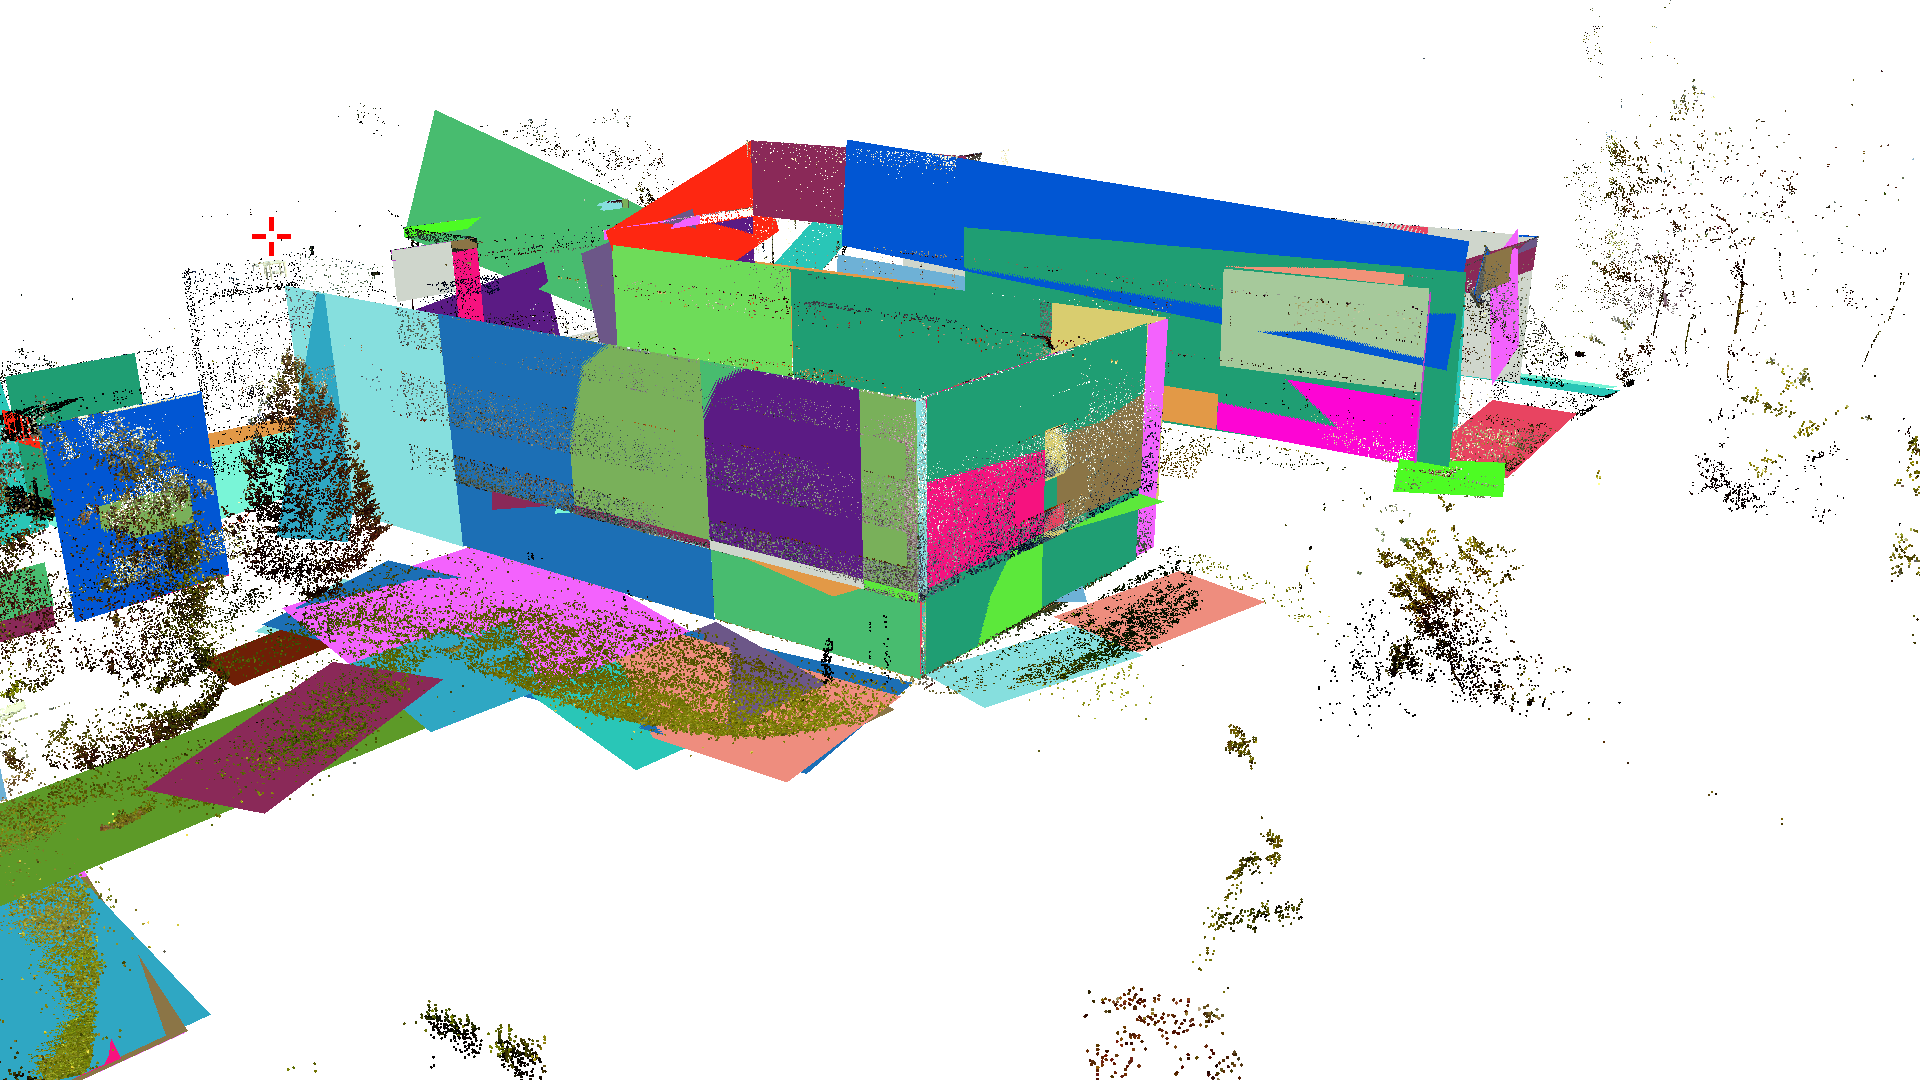
\includegraphics[width=0.7\textwidth]{Results/technologiezentrum_shapes_interactive.png}%
  }
\caption[Figure (a) shows a rendering og the Technologiezentrum dataset, (b) shows the resulting shapes of the RANSAC shape detection, (c) shows the result of the interactive shape detection.]
{Figure (a) shows a rendering of the Technologiezentrum dataset, (b) shows the resulting shapes of the RANSAC shape detection, (c) shows the detected shapes using the interactive shape detection method.}

\label{fig:technologiezentrum_results}
\end{figure}


\begin{figure}
\centering
\subcaptionbox{ \label{fig:technologiezentrum_interactive_shape_detection1}}{%
  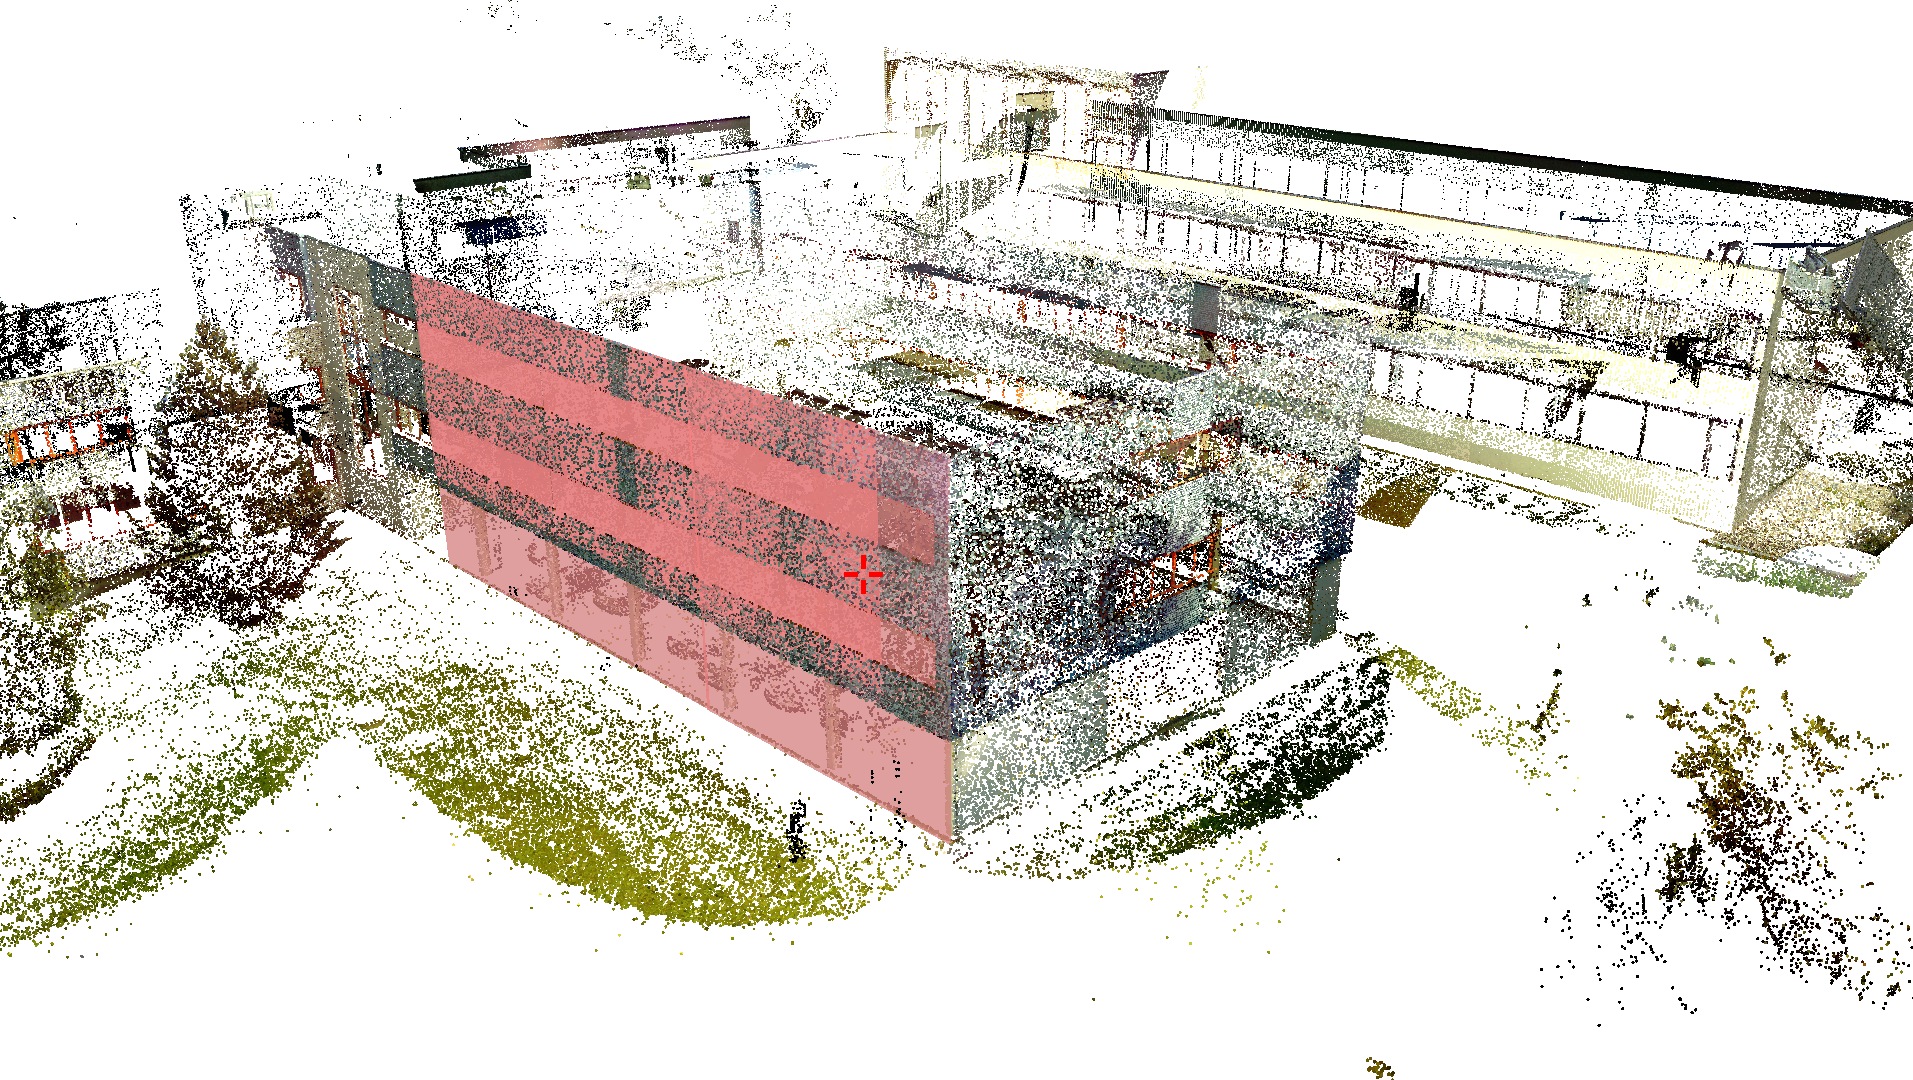
\includegraphics[width=\textwidth]{Results/technologiezentrum_interactive_shape_detection1.png}%7
  }
\subcaptionbox{ \label{fig:technologiezentrum_interactive_shape_detection2}}{%
  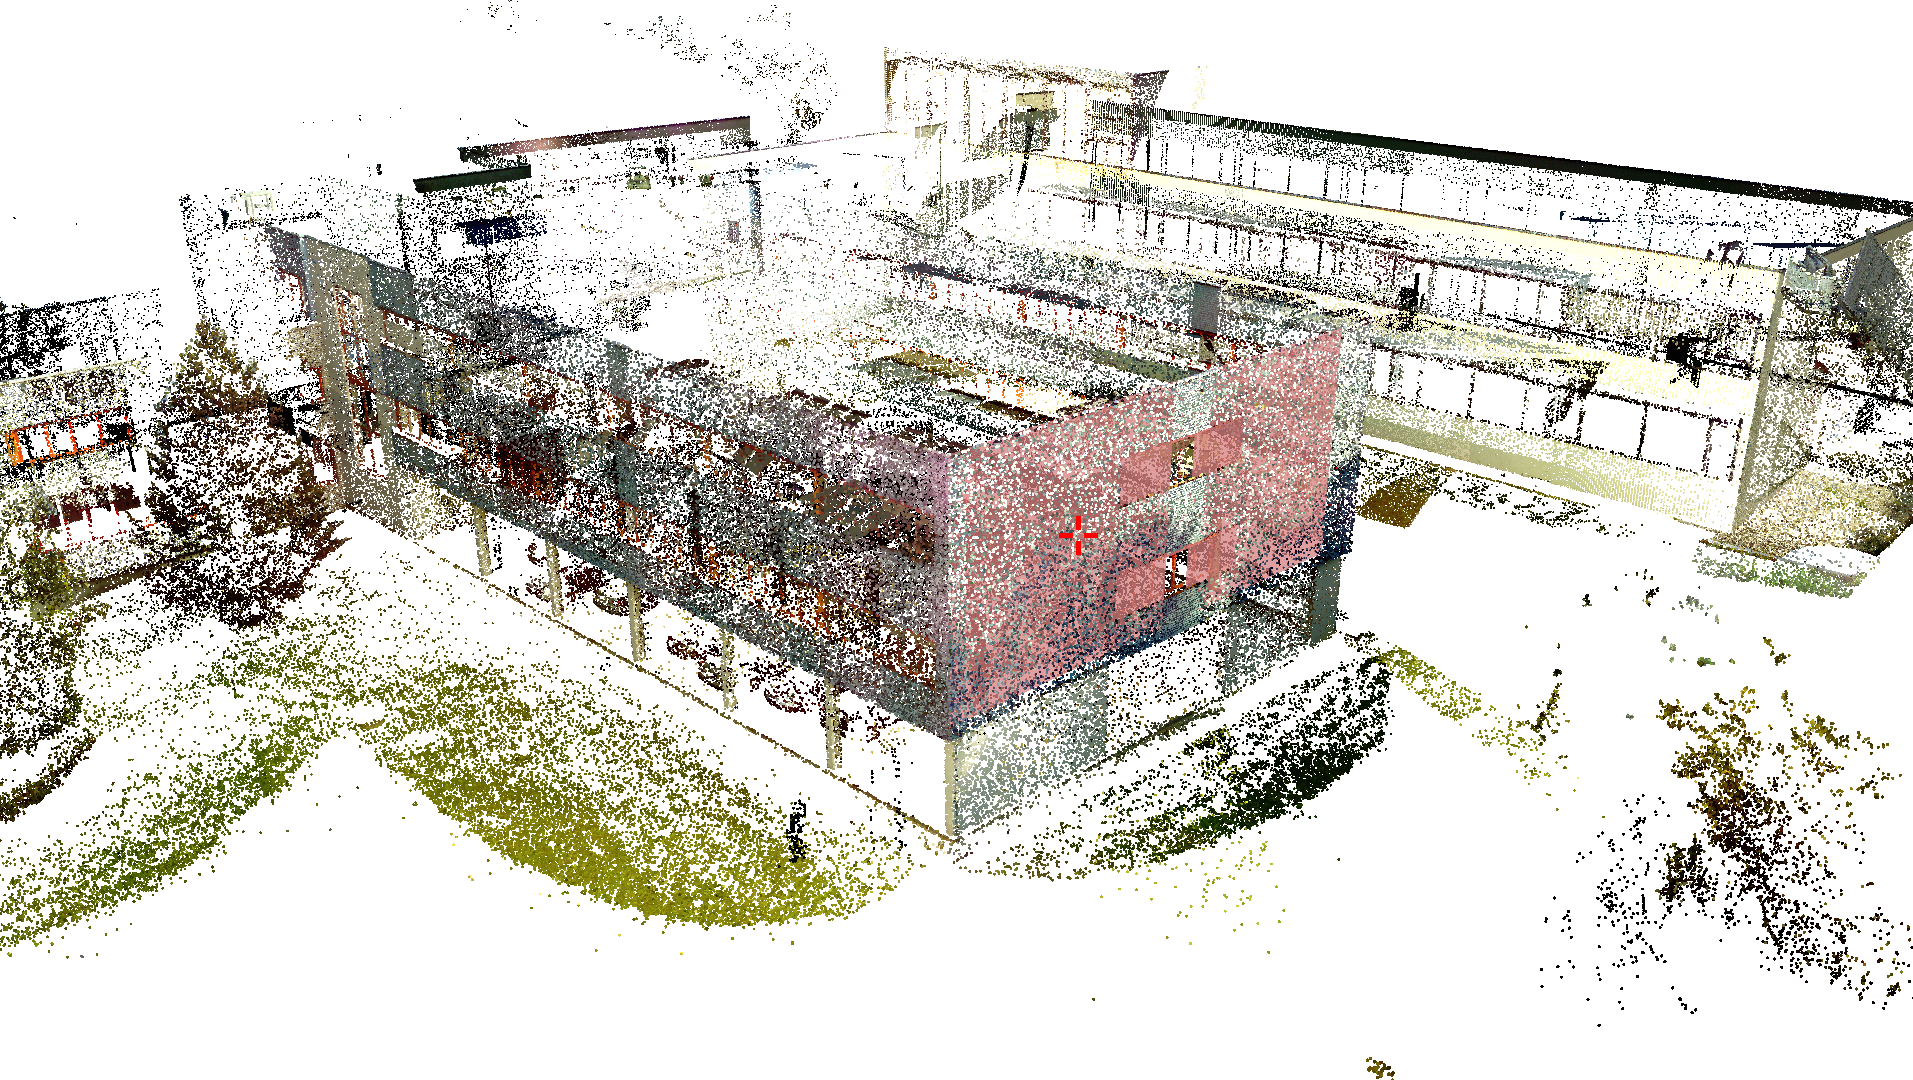
\includegraphics[width=\textwidth]{Results/technologiezentrum_interactive_shape_detection2.png}%
  }
\caption[Two examples of user-guided shape detection]
{This figure shows a rendering of the Technologiezentrum dataset. Based on the cursor's position (indicated as the red cross hair) a different shape are selected. The shape is rendered in red. (a) and (b) show different shapes for different parts of the point cloud. Both shapes are a part of a wall.}
\label{fig:technologiezentrum_interactive_shape_detection}
\end{figure}


\section{Interaction Results}
\label{sec:interaction_results}

This section presents a set of figures that showcase the different interactions from Section \ref{sec:interactions}. The interactions are performed on the Technologiezentrum dataset since the JB\_Haus point cloud is used as an example throughout this thesis already. 

\begin{figure}[h]
\centering
\subcaptionbox{ \label{fig:technologiezentrum_lasso1}}{%
  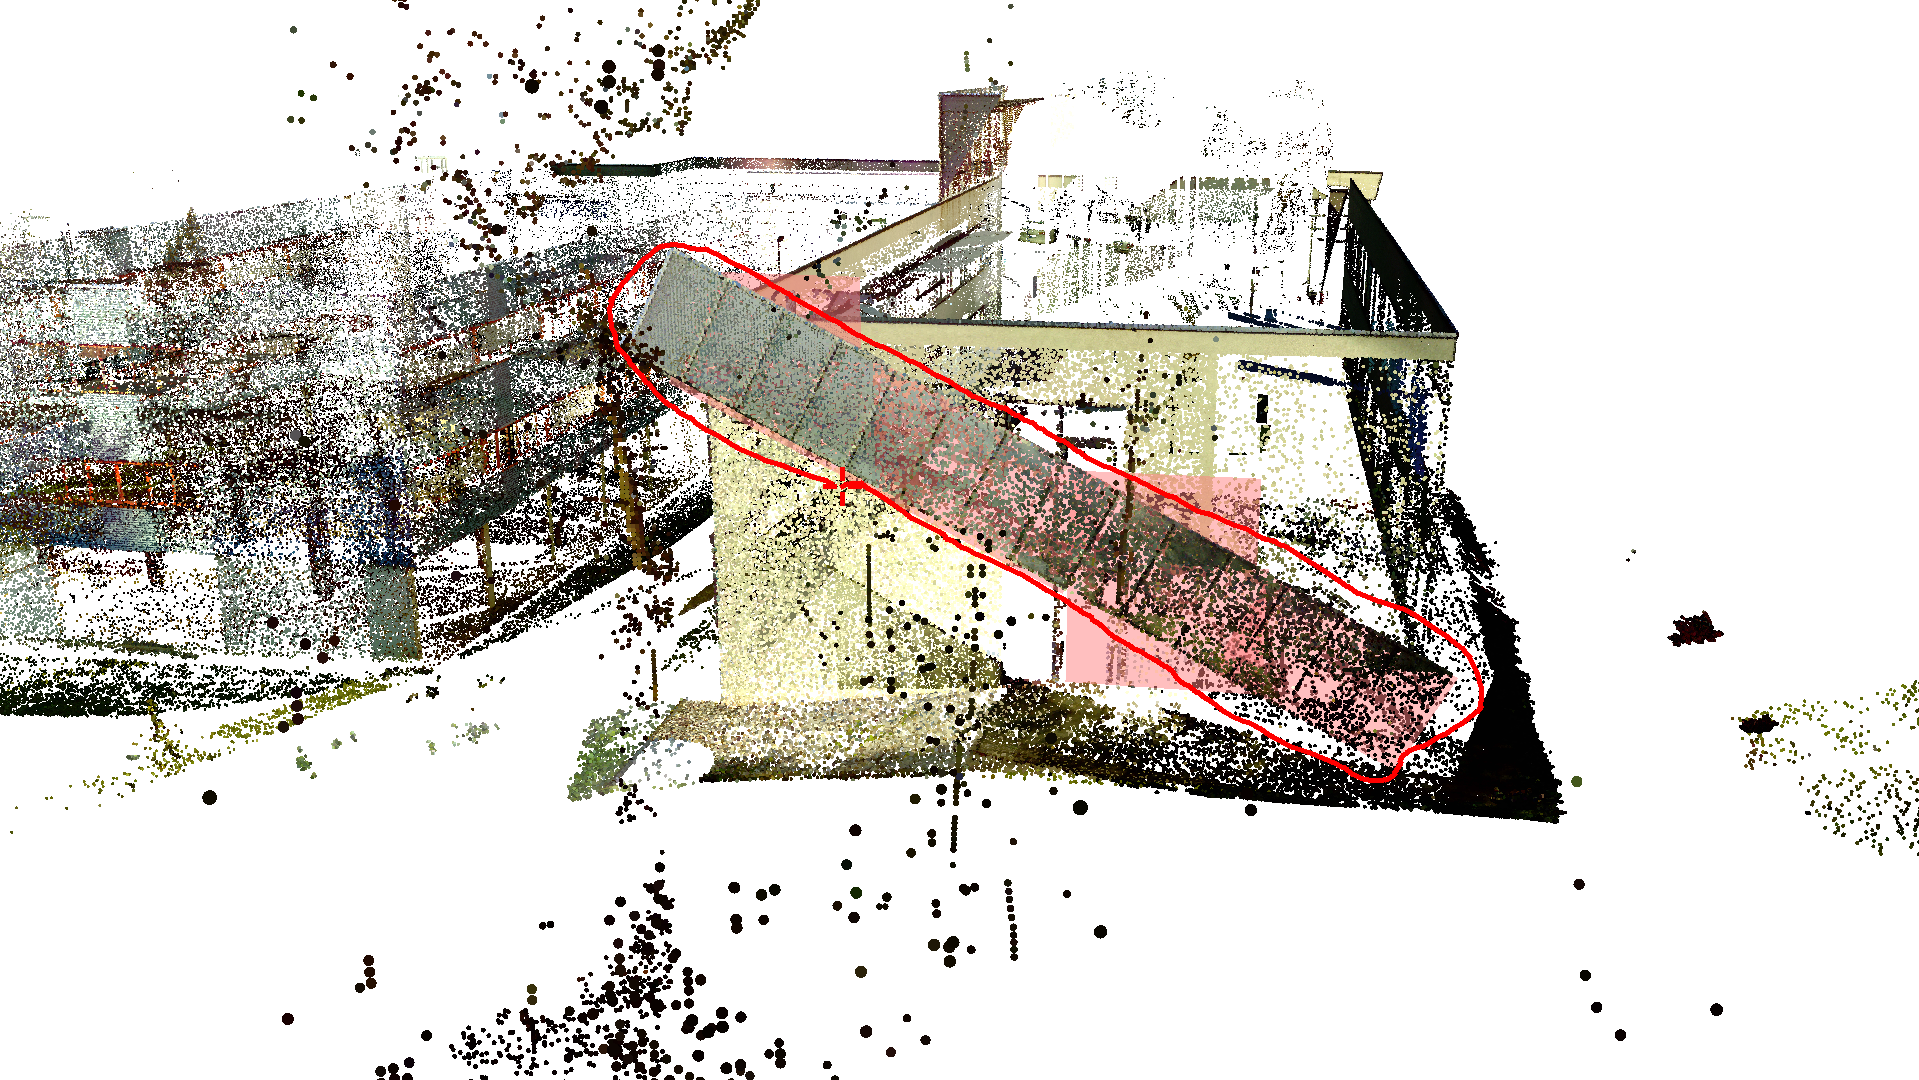
\includegraphics[width=0.9\textwidth]{Results/technologiezentrum_lasso1.png}%7
  }
\subcaptionbox{ \label{fig:technologiezentrum_lasso2}}{%
  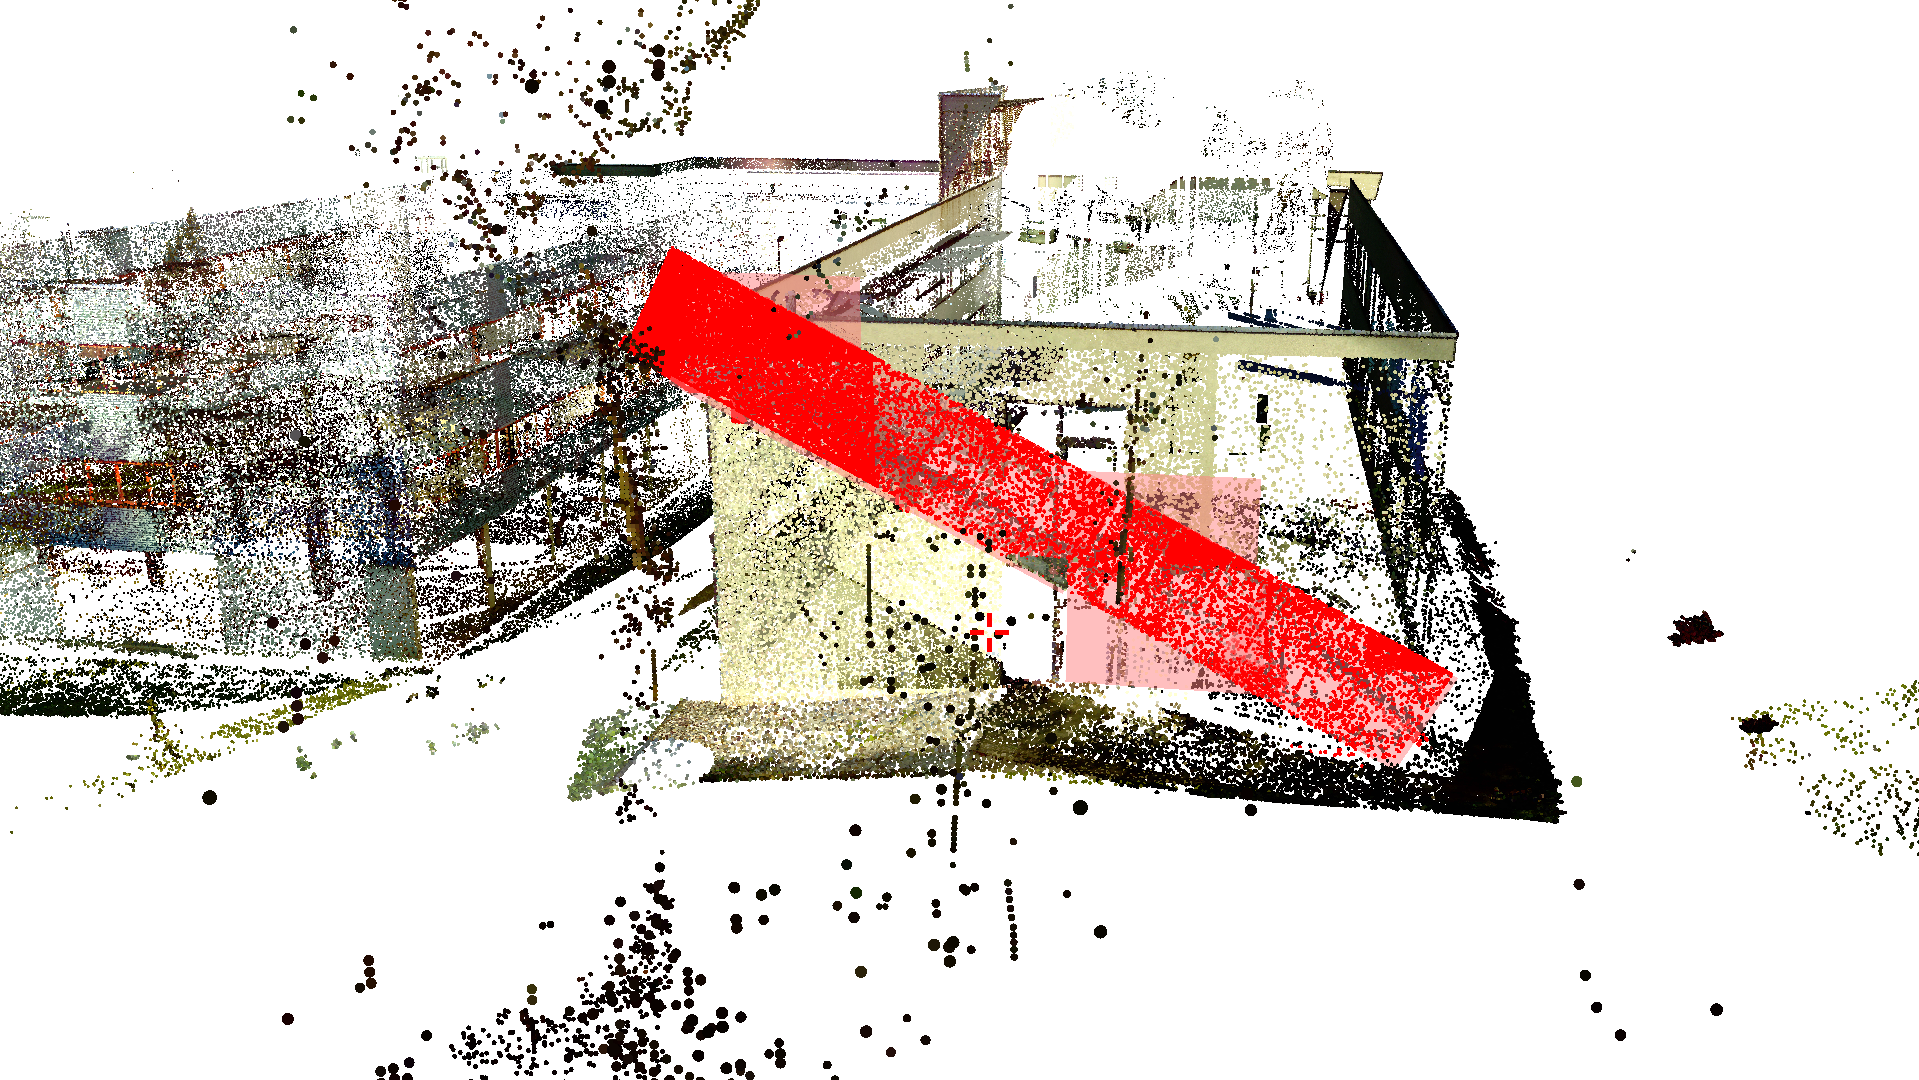
\includegraphics[width=0.9\textwidth]{Results/technologiezentrum_lasso2.png}%
  }
\caption[Example of an improved lasso selection]
{A lasso selection is performed on the selected support shape in (a). Only points are selected that lie on the support shape as shown in (b). Point in front and back of the support shape are not selected. }
\label{fig:technologiezentrum_lasso}
\end{figure}


\begin{figure}
\centering
\subcaptionbox{ \label{fig:technologiezentrum_brush1}}{%
  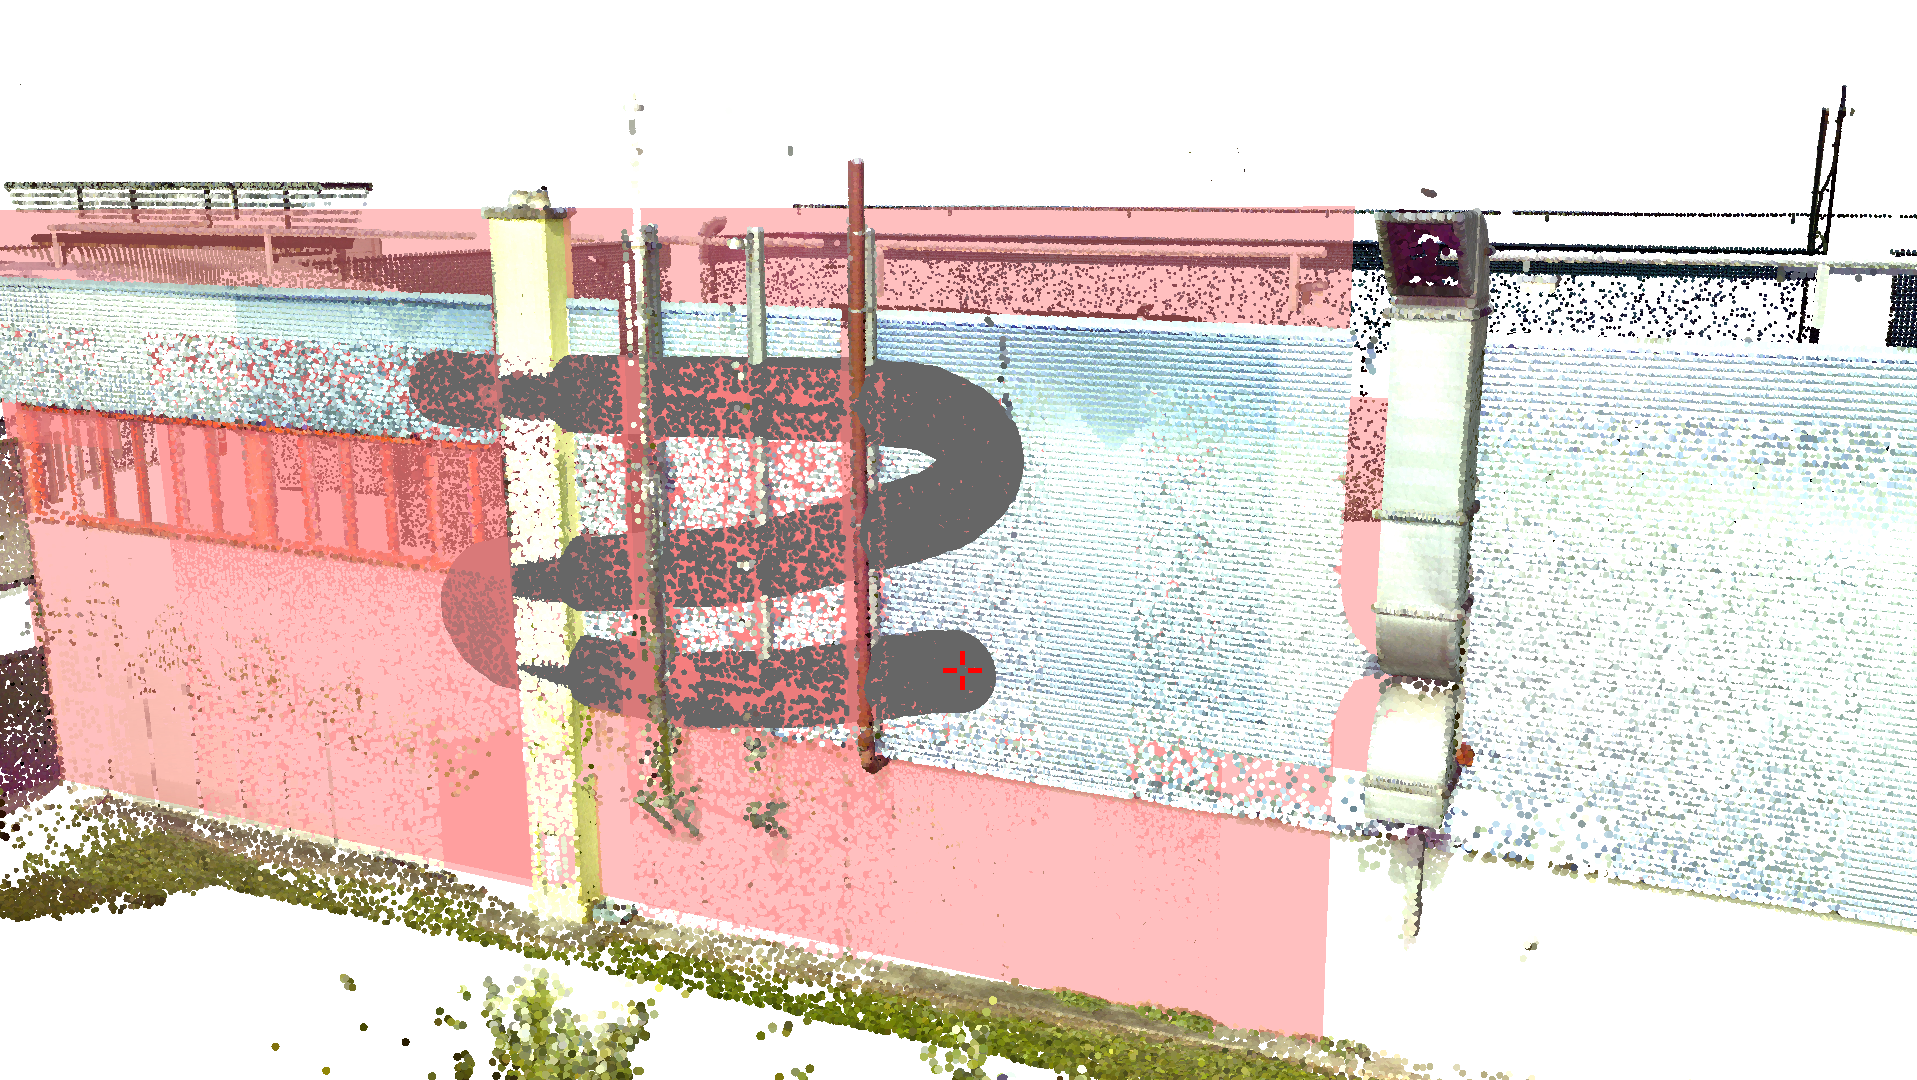
\includegraphics[width=\textwidth]{Results/technologiezentrum_brush1.png}%7
  }
\subcaptionbox{ \label{fig:technologiezentrum_brush2}}{%
  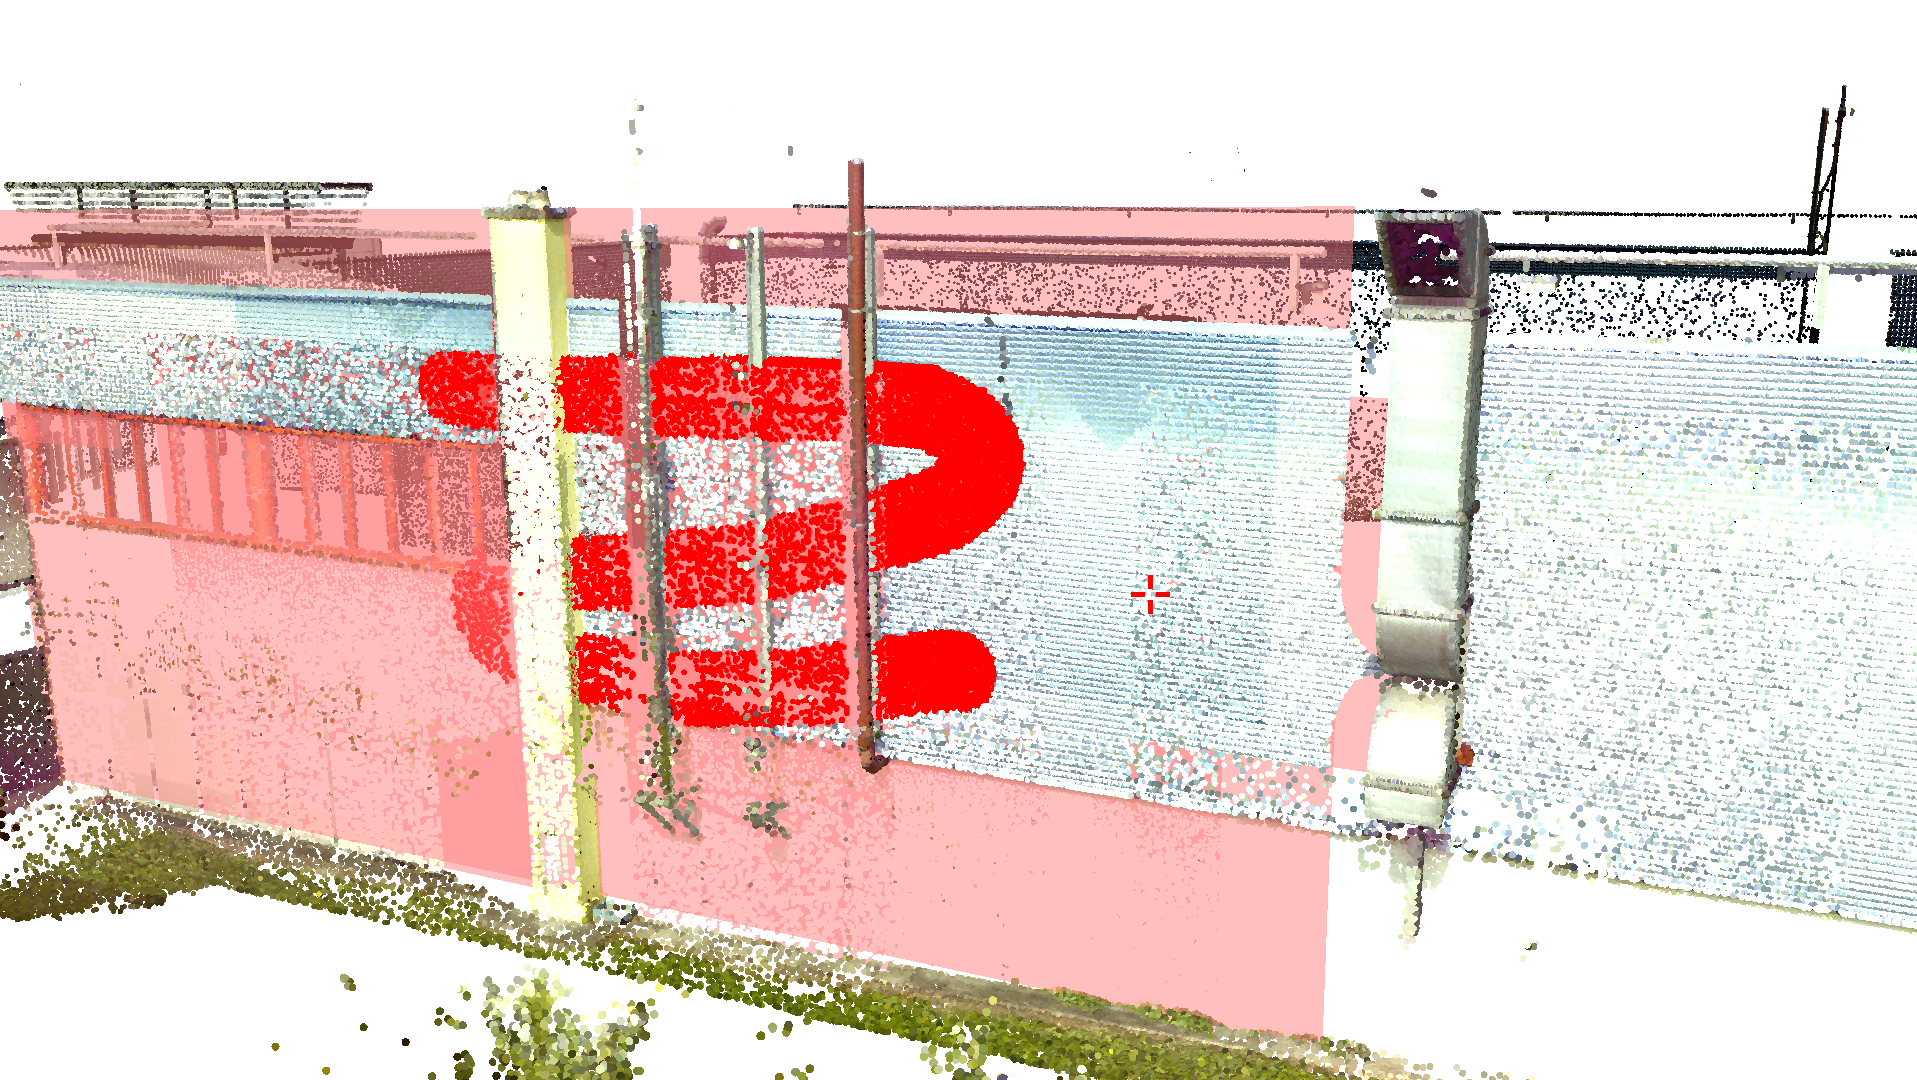
\includegraphics[width=\textwidth]{Results/technologiezentrum_brush2.png}%
  }
\caption[Example of an improved volumetric brush selection]
{A volumetric brush selection is performed on the selected support shape in (a). Point are only selected if they belong to the support shape and intersect the brush. The result of the selection can be seen in (b).}
\label{fig:technologiezentrum_brush}
\end{figure}


\begin{figure}
\centering
\subcaptionbox{ \label{fig:technologiezentrum_lod_increment1}}{%
  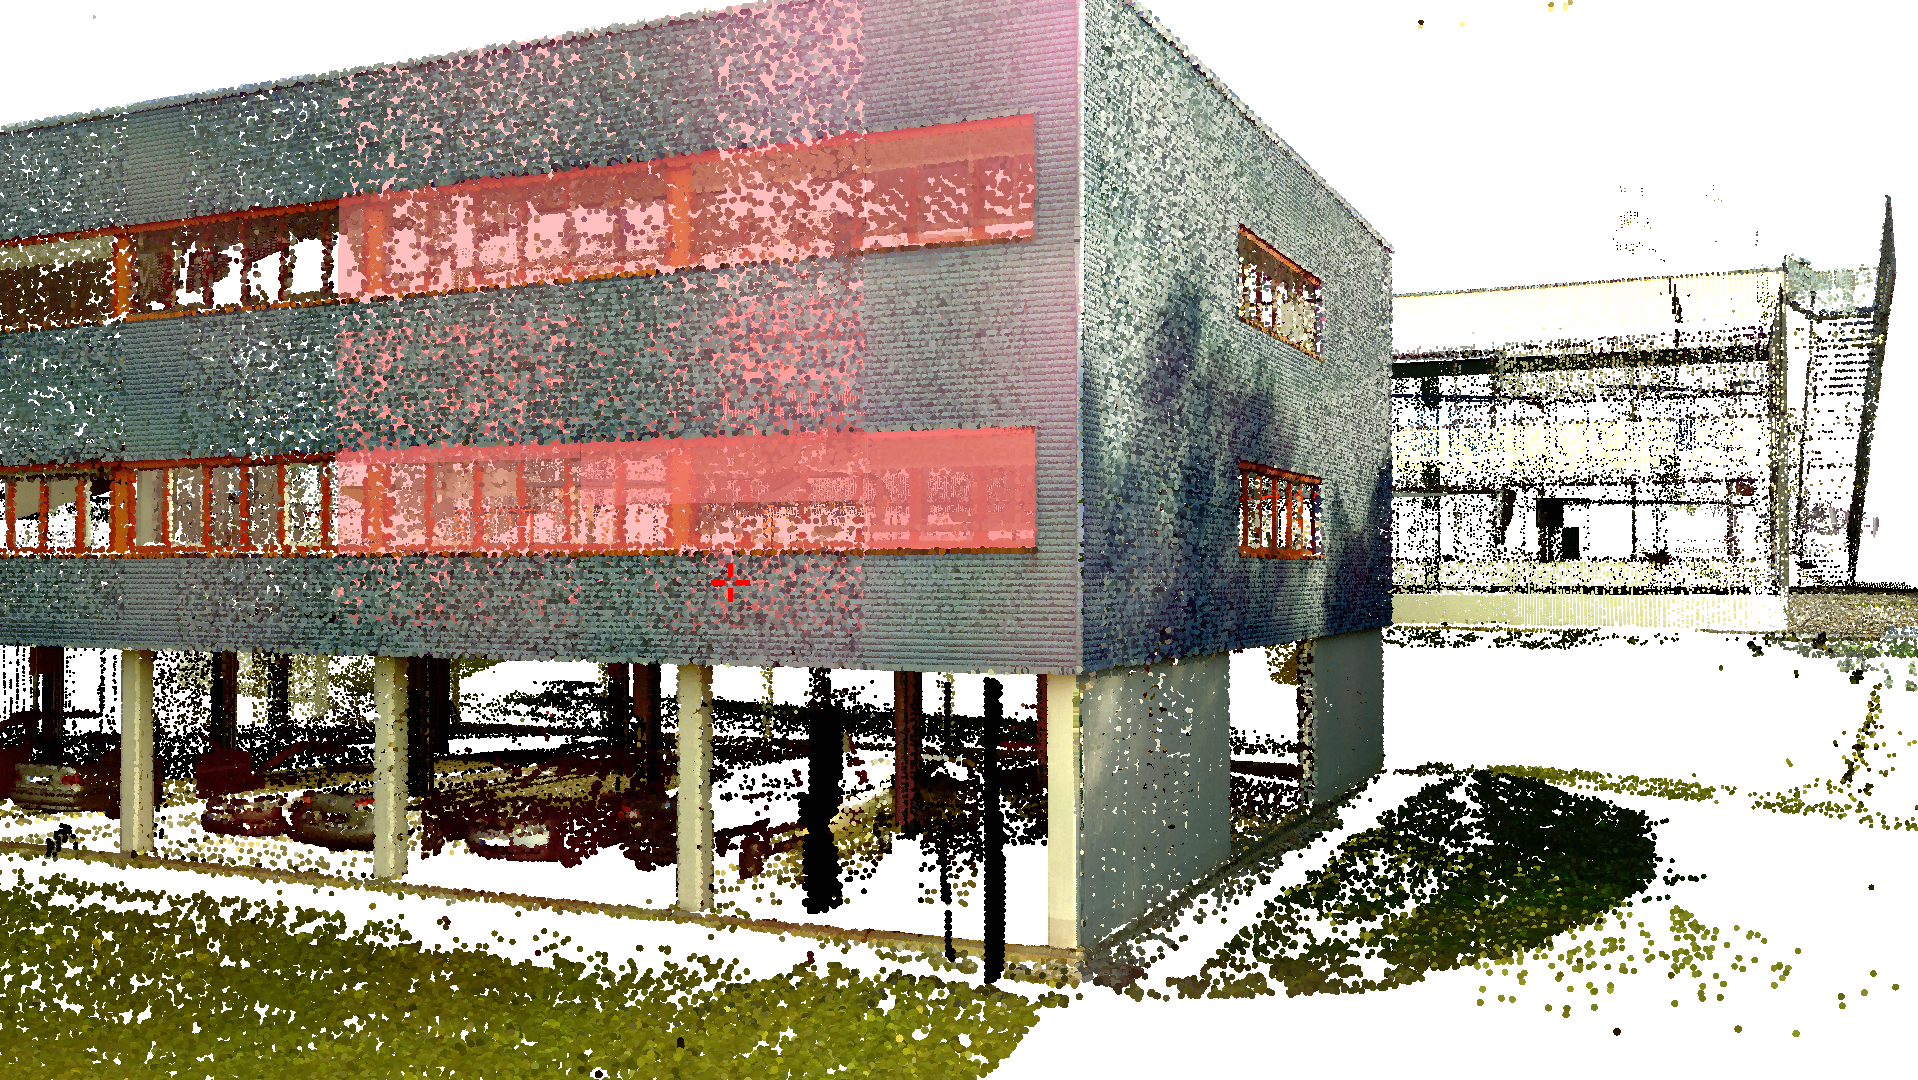
\includegraphics[width=\textwidth]{Results/technologiezentrum_lod_increment1.png}%7
  }
\subcaptionbox{ \label{fig:technologiezentrum_lod_increment2}}{%
  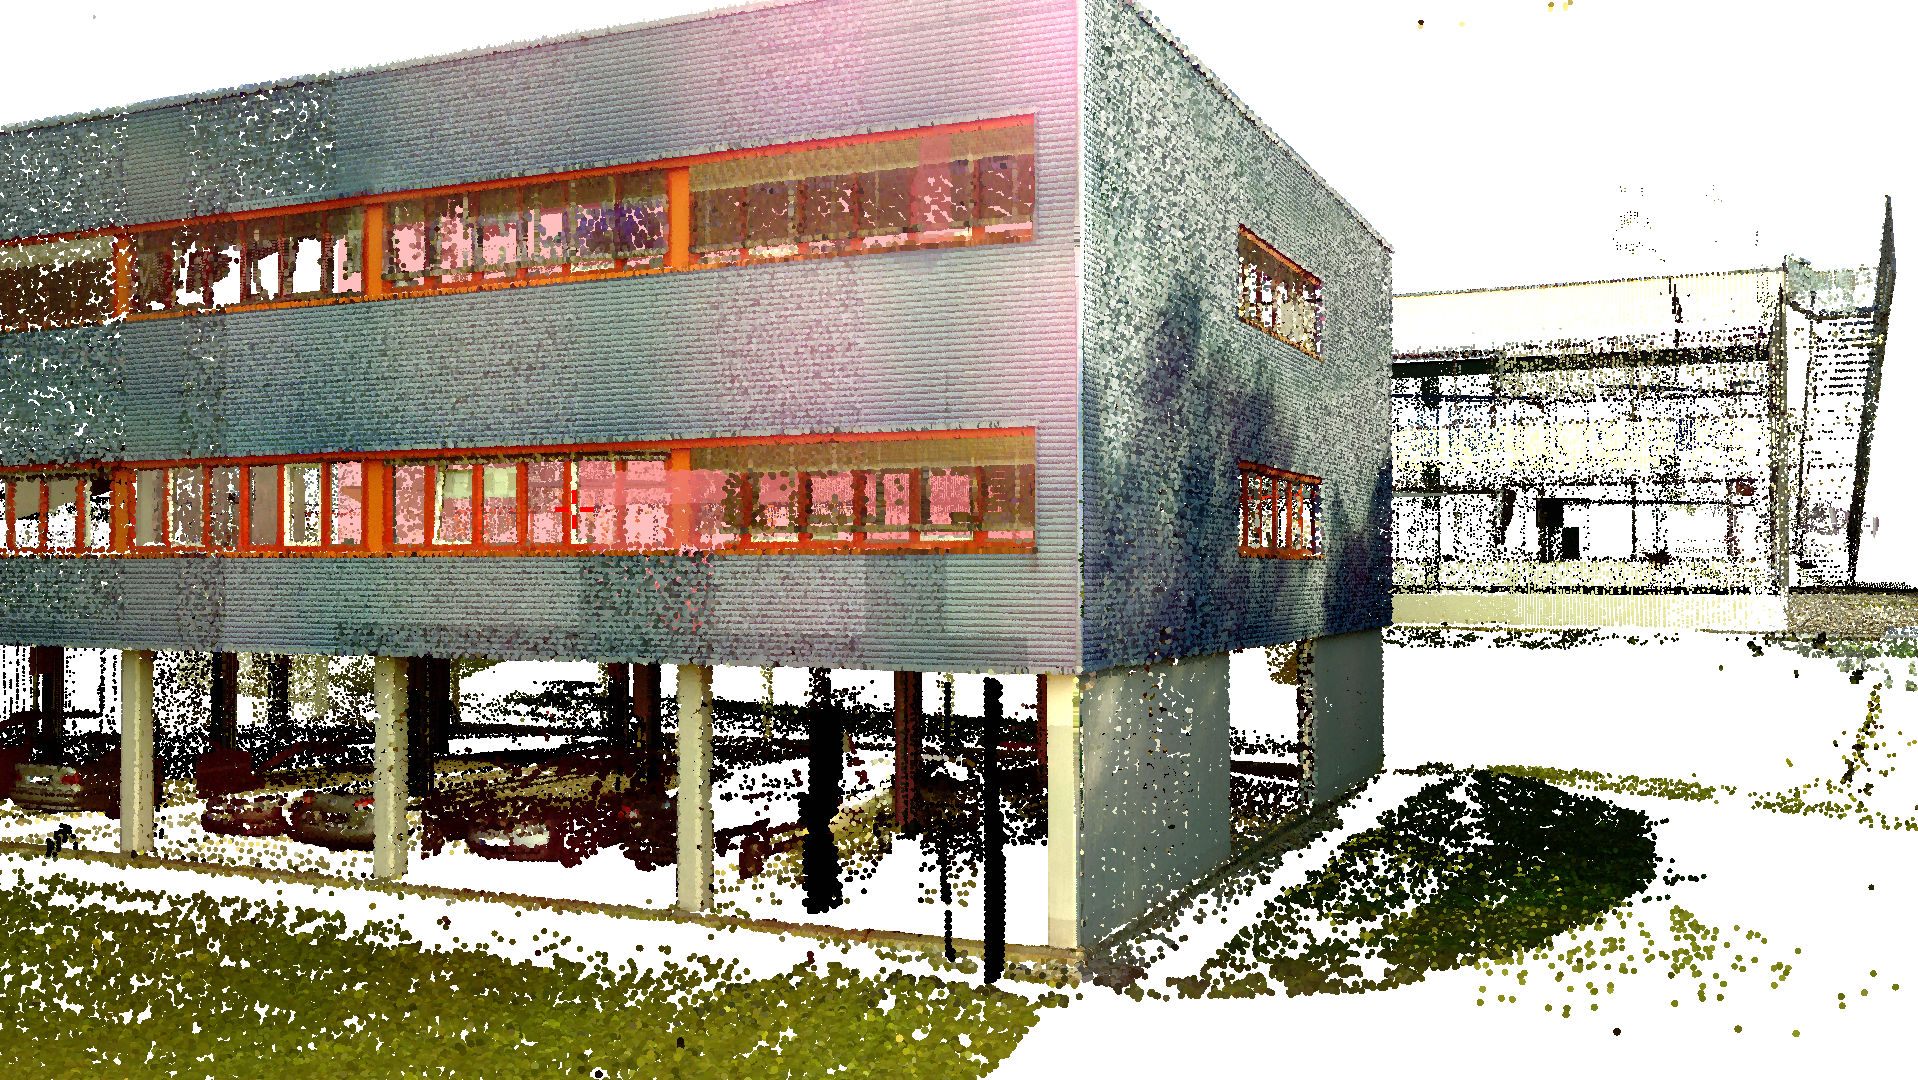
\includegraphics[width=\textwidth]{Results/technologiezentrum_lod_increment2.png}%
  }
\caption[Example of the local increment of level-of-detail]
{This figure shows the lcaol increment of the level-of-detail. The level-of-detail is incremented along the support shape. (a) shows the original rendering model of the point cloud, (b) shows the point cloud with additional points. }
\label{fig:technologiezentrum_lod_increment}
\end{figure}


% Examples for non-planar shapes

\begin{figure}
\centering
\subcaptionbox{ \label{fig:syntheticScene_lasso1}}{%
  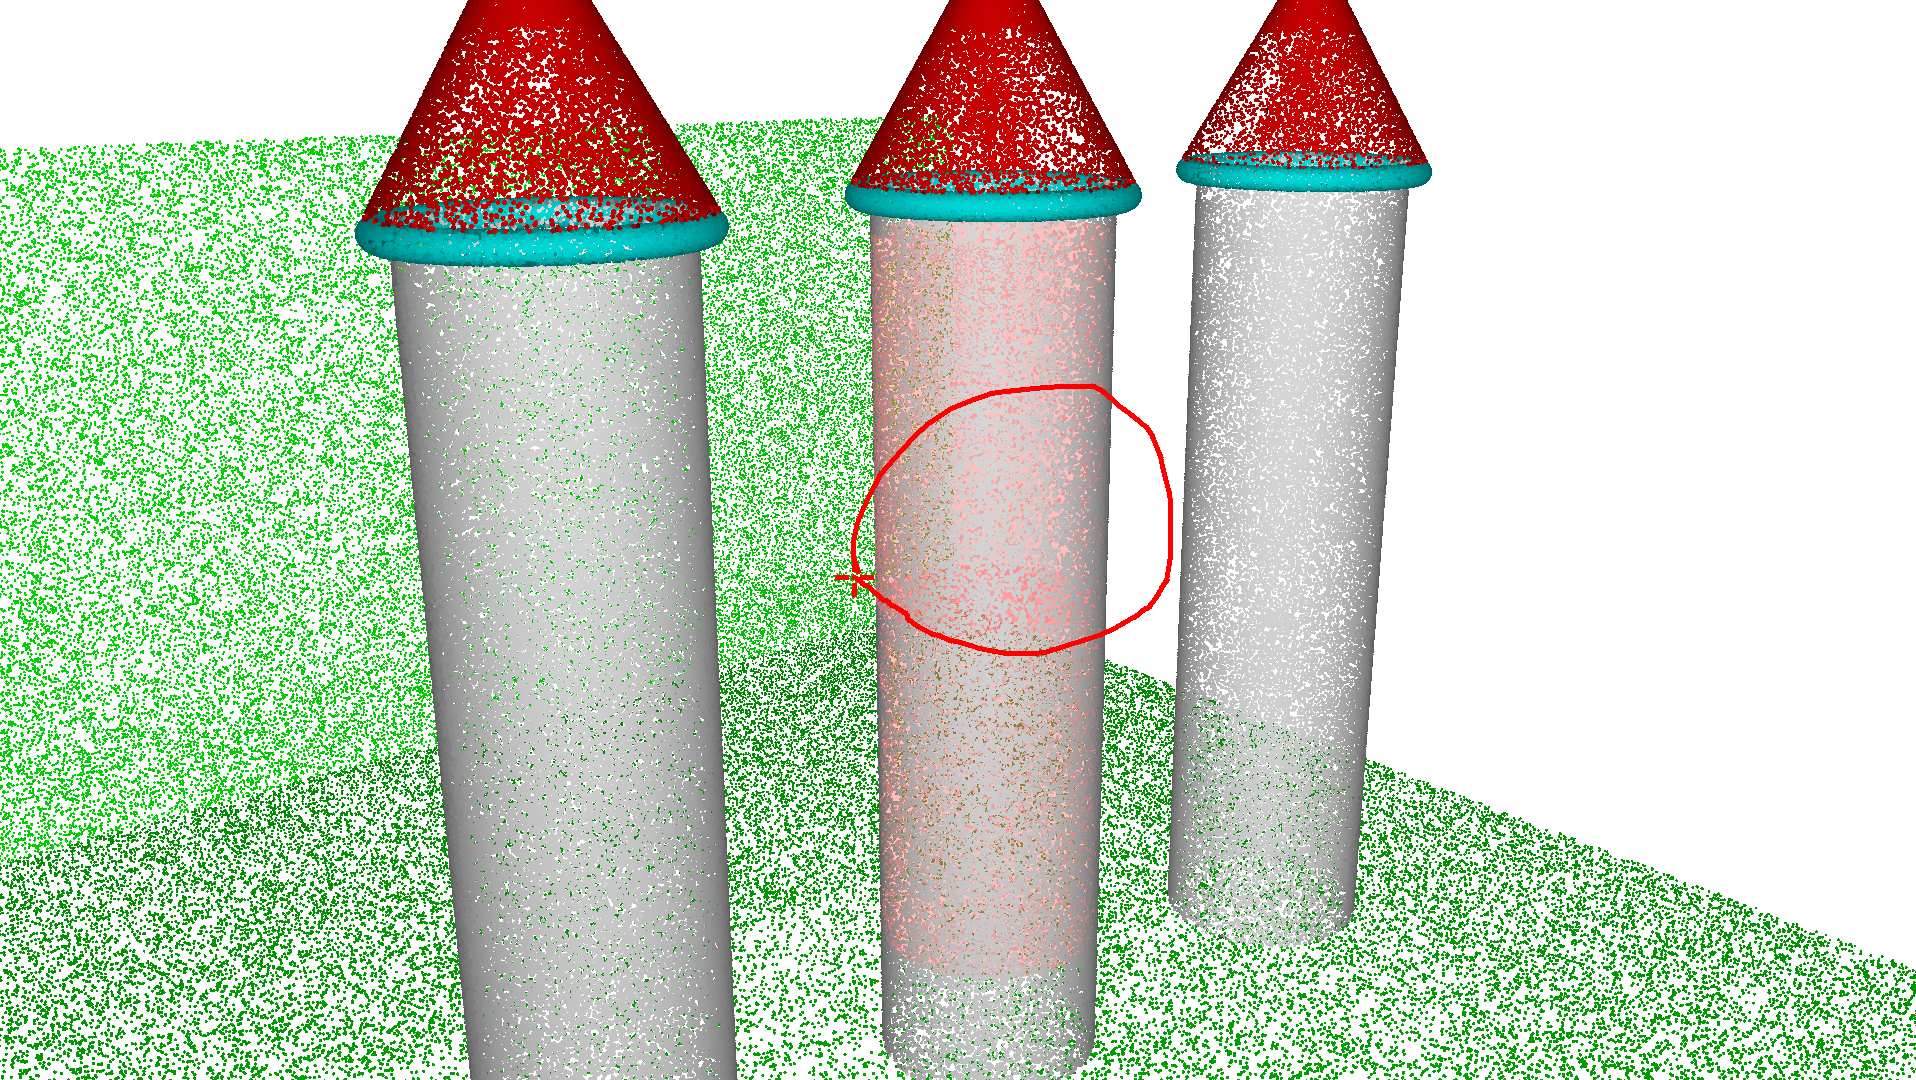
\includegraphics[width=\textwidth]{Results/synthetic_point_cloud_lasso1.png}%7
  }
\subcaptionbox{ \label{fig:syntheticScene_lasso2}}{%
  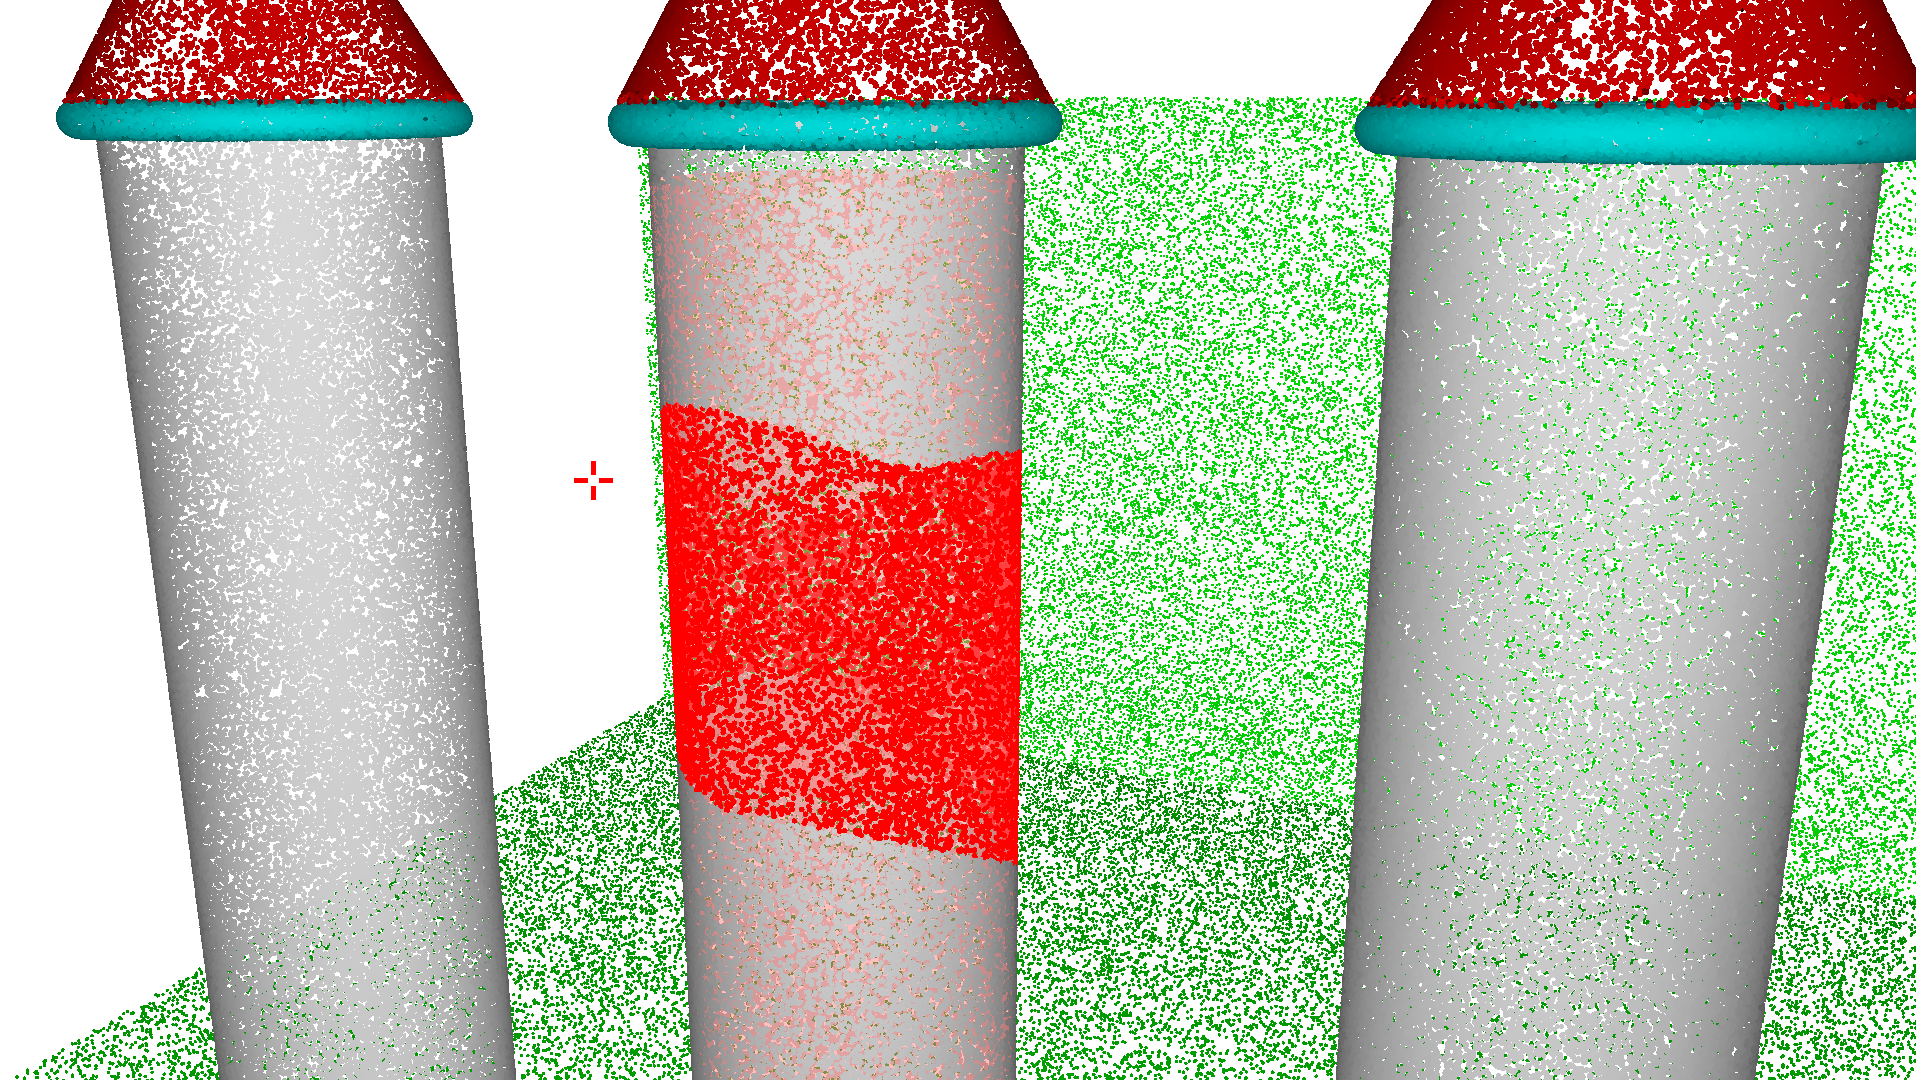
\includegraphics[width=\textwidth]{Results/synthetic_point_cloud_lasso2.png}%
  }
\caption[Example of an improved lasso selection on a cylinder]
{This figure shows an improved lasso selection performed using a cylinder shape as support. (a) shows the lasso that is drawn on screen, (b) shows the selection result from a different angle. Points in the back of the cylinder are selected as well, as they are approximated by the cylinder as well. }
\label{fig:syntheticScene_lasso}
\end{figure}


\begin{figure}
\centering
\subcaptionbox{ \label{fig:syntheticScene_brush1}}{%
  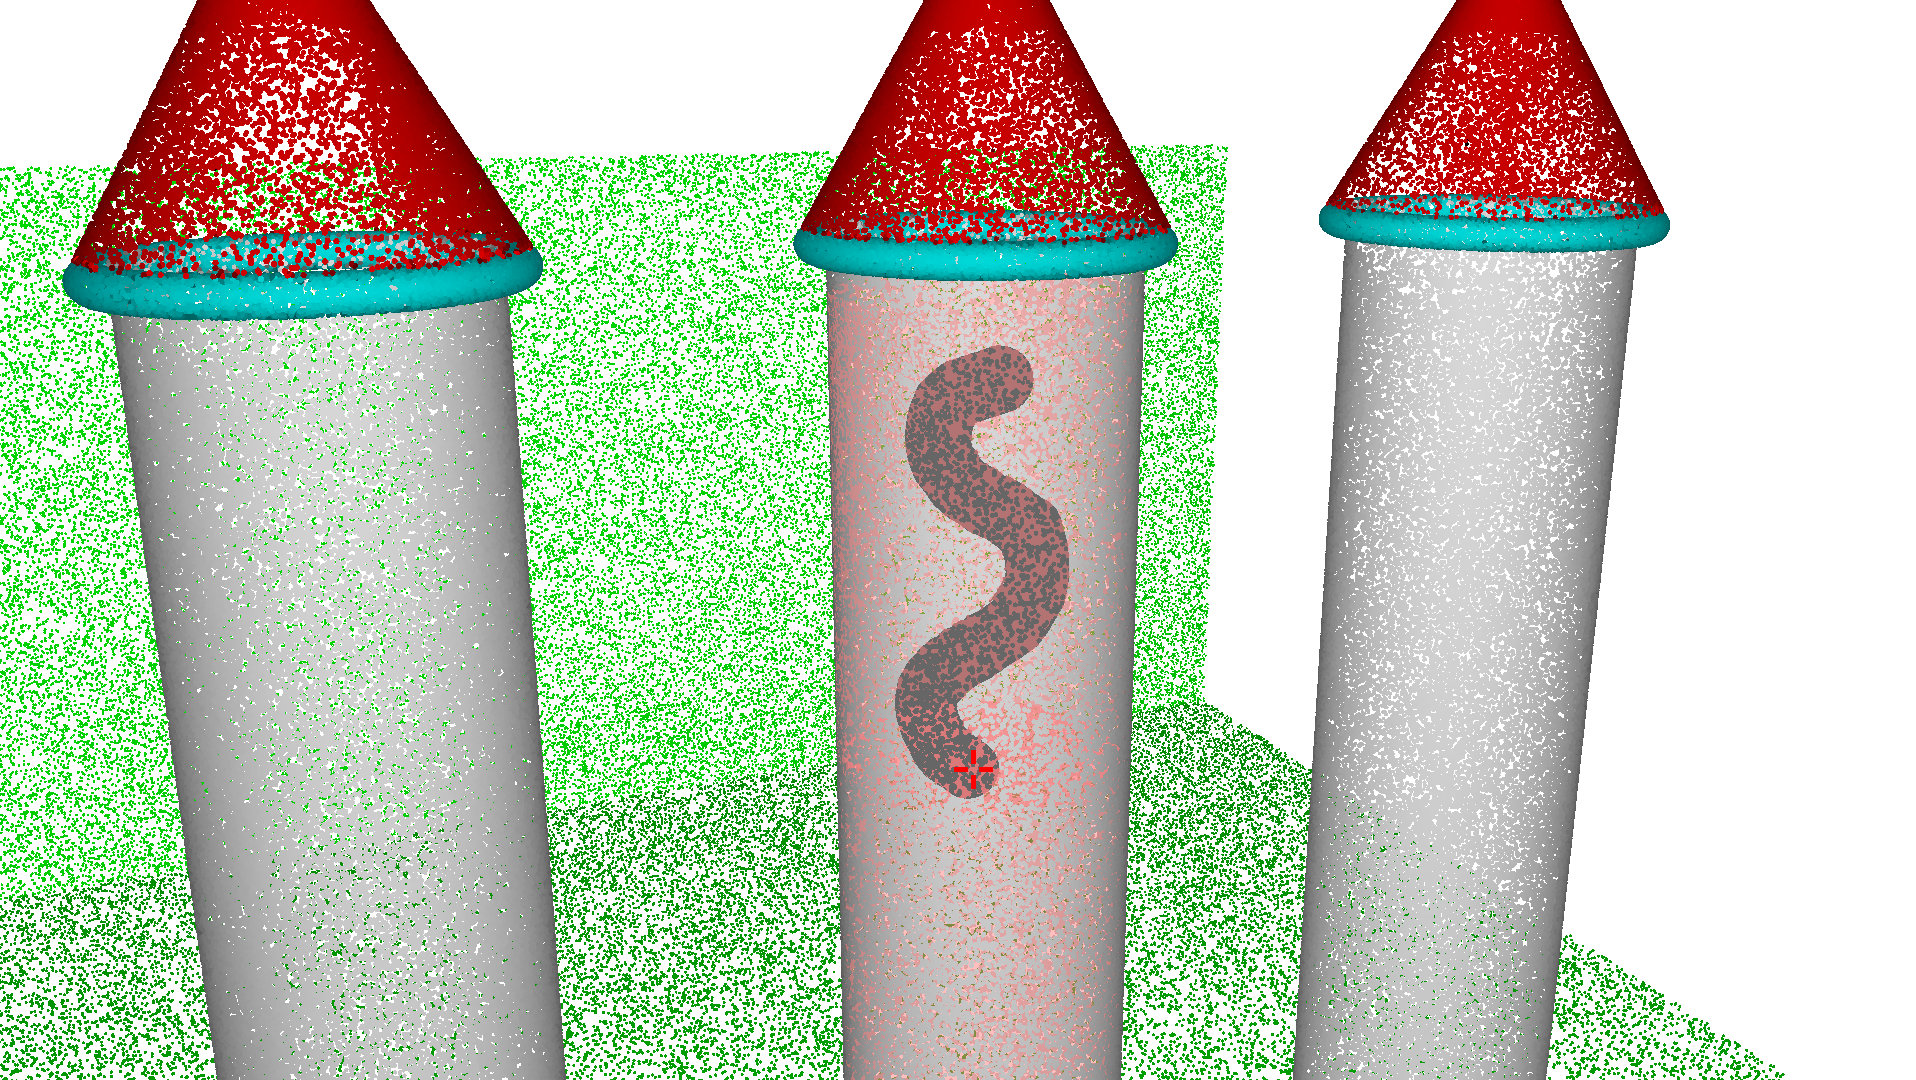
\includegraphics[width=\textwidth]{Results/synthetic_point_cloud_brush1.png}%7
  }
\subcaptionbox{ \label{fig:syntheticScene_brush2}}{%
  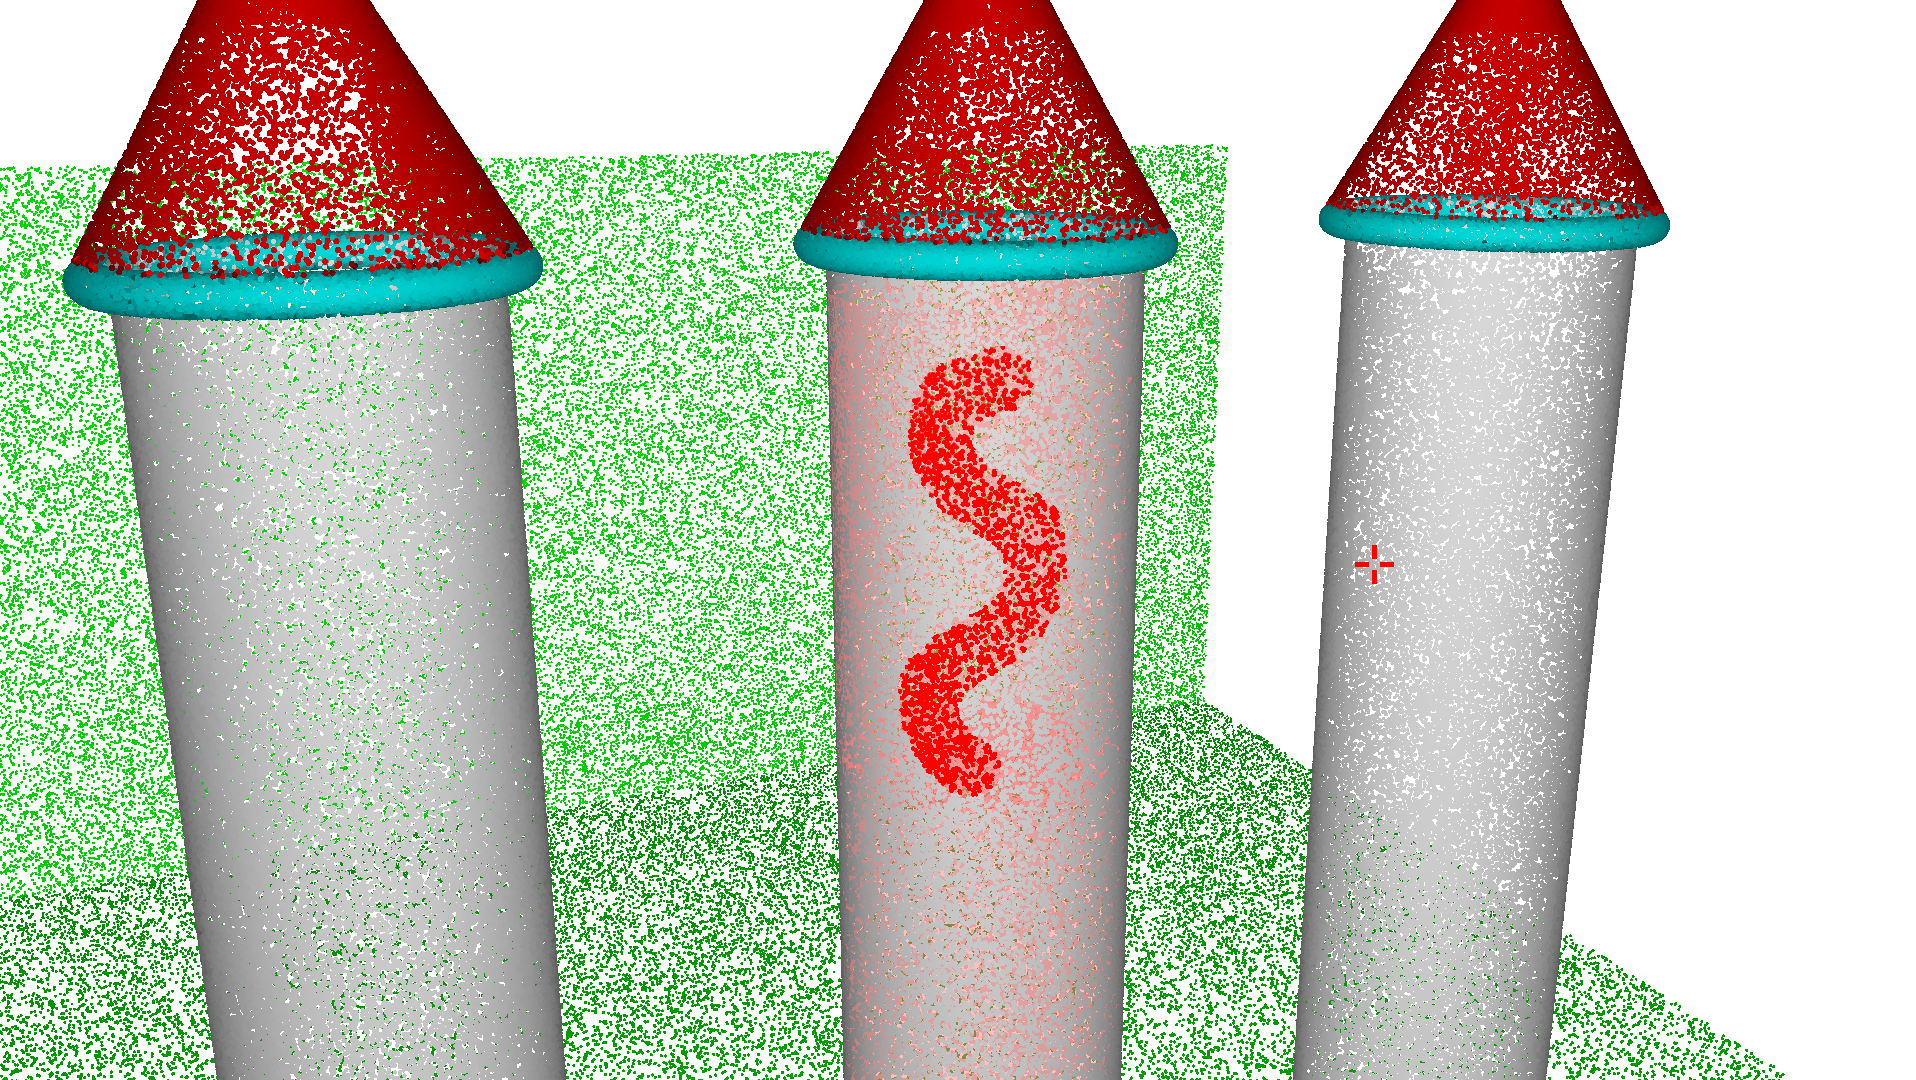
\includegraphics[width=\textwidth]{Results/synthetic_point_cloud_brush2.png}%
  }
\caption[Example of an improved volumetric brush selection on a cylinder]
{This figure shows the volumetric brush selection on a selected cylinder shape. The brush sticks to the side of the cylinder that is facing the camera.}
\label{fig:syntheticScene_brush}
\end{figure}